\documentclass[]{article}
\usepackage{lmodern}
\usepackage{amssymb,amsmath}
\usepackage{ifxetex,ifluatex}
\usepackage{fixltx2e} % provides \textsubscript
\ifnum 0\ifxetex 1\fi\ifluatex 1\fi=0 % if pdftex
  \usepackage[T1]{fontenc}
  \usepackage[utf8]{inputenc}
\else % if luatex or xelatex
  \ifxetex
    \usepackage{mathspec}
  \else
    \usepackage{fontspec}
  \fi
  \defaultfontfeatures{Ligatures=TeX,Scale=MatchLowercase}
\fi
% use upquote if available, for straight quotes in verbatim environments
\IfFileExists{upquote.sty}{\usepackage{upquote}}{}
% use microtype if available
\IfFileExists{microtype.sty}{%
\usepackage{microtype}
\UseMicrotypeSet[protrusion]{basicmath} % disable protrusion for tt fonts
}{}
\usepackage[margin=1in]{geometry}
\usepackage{hyperref}
\hypersetup{unicode=true,
            pdftitle={Liver Disease Classification},
            pdfauthor={Nabeel Khan},
            pdfborder={0 0 0},
            breaklinks=true}
\urlstyle{same}  % don't use monospace font for urls
\usepackage{color}
\usepackage{fancyvrb}
\newcommand{\VerbBar}{|}
\newcommand{\VERB}{\Verb[commandchars=\\\{\}]}
\DefineVerbatimEnvironment{Highlighting}{Verbatim}{commandchars=\\\{\}}
% Add ',fontsize=\small' for more characters per line
\usepackage{framed}
\definecolor{shadecolor}{RGB}{248,248,248}
\newenvironment{Shaded}{\begin{snugshade}}{\end{snugshade}}
\newcommand{\AlertTok}[1]{\textcolor[rgb]{0.94,0.16,0.16}{#1}}
\newcommand{\AnnotationTok}[1]{\textcolor[rgb]{0.56,0.35,0.01}{\textbf{\textit{#1}}}}
\newcommand{\AttributeTok}[1]{\textcolor[rgb]{0.77,0.63,0.00}{#1}}
\newcommand{\BaseNTok}[1]{\textcolor[rgb]{0.00,0.00,0.81}{#1}}
\newcommand{\BuiltInTok}[1]{#1}
\newcommand{\CharTok}[1]{\textcolor[rgb]{0.31,0.60,0.02}{#1}}
\newcommand{\CommentTok}[1]{\textcolor[rgb]{0.56,0.35,0.01}{\textit{#1}}}
\newcommand{\CommentVarTok}[1]{\textcolor[rgb]{0.56,0.35,0.01}{\textbf{\textit{#1}}}}
\newcommand{\ConstantTok}[1]{\textcolor[rgb]{0.00,0.00,0.00}{#1}}
\newcommand{\ControlFlowTok}[1]{\textcolor[rgb]{0.13,0.29,0.53}{\textbf{#1}}}
\newcommand{\DataTypeTok}[1]{\textcolor[rgb]{0.13,0.29,0.53}{#1}}
\newcommand{\DecValTok}[1]{\textcolor[rgb]{0.00,0.00,0.81}{#1}}
\newcommand{\DocumentationTok}[1]{\textcolor[rgb]{0.56,0.35,0.01}{\textbf{\textit{#1}}}}
\newcommand{\ErrorTok}[1]{\textcolor[rgb]{0.64,0.00,0.00}{\textbf{#1}}}
\newcommand{\ExtensionTok}[1]{#1}
\newcommand{\FloatTok}[1]{\textcolor[rgb]{0.00,0.00,0.81}{#1}}
\newcommand{\FunctionTok}[1]{\textcolor[rgb]{0.00,0.00,0.00}{#1}}
\newcommand{\ImportTok}[1]{#1}
\newcommand{\InformationTok}[1]{\textcolor[rgb]{0.56,0.35,0.01}{\textbf{\textit{#1}}}}
\newcommand{\KeywordTok}[1]{\textcolor[rgb]{0.13,0.29,0.53}{\textbf{#1}}}
\newcommand{\NormalTok}[1]{#1}
\newcommand{\OperatorTok}[1]{\textcolor[rgb]{0.81,0.36,0.00}{\textbf{#1}}}
\newcommand{\OtherTok}[1]{\textcolor[rgb]{0.56,0.35,0.01}{#1}}
\newcommand{\PreprocessorTok}[1]{\textcolor[rgb]{0.56,0.35,0.01}{\textit{#1}}}
\newcommand{\RegionMarkerTok}[1]{#1}
\newcommand{\SpecialCharTok}[1]{\textcolor[rgb]{0.00,0.00,0.00}{#1}}
\newcommand{\SpecialStringTok}[1]{\textcolor[rgb]{0.31,0.60,0.02}{#1}}
\newcommand{\StringTok}[1]{\textcolor[rgb]{0.31,0.60,0.02}{#1}}
\newcommand{\VariableTok}[1]{\textcolor[rgb]{0.00,0.00,0.00}{#1}}
\newcommand{\VerbatimStringTok}[1]{\textcolor[rgb]{0.31,0.60,0.02}{#1}}
\newcommand{\WarningTok}[1]{\textcolor[rgb]{0.56,0.35,0.01}{\textbf{\textit{#1}}}}
\usepackage{longtable,booktabs}
\usepackage{graphicx,grffile}
\makeatletter
\def\maxwidth{\ifdim\Gin@nat@width>\linewidth\linewidth\else\Gin@nat@width\fi}
\def\maxheight{\ifdim\Gin@nat@height>\textheight\textheight\else\Gin@nat@height\fi}
\makeatother
% Scale images if necessary, so that they will not overflow the page
% margins by default, and it is still possible to overwrite the defaults
% using explicit options in \includegraphics[width, height, ...]{}
\setkeys{Gin}{width=\maxwidth,height=\maxheight,keepaspectratio}
\IfFileExists{parskip.sty}{%
\usepackage{parskip}
}{% else
\setlength{\parindent}{0pt}
\setlength{\parskip}{6pt plus 2pt minus 1pt}
}
\setlength{\emergencystretch}{3em}  % prevent overfull lines
\providecommand{\tightlist}{%
  \setlength{\itemsep}{0pt}\setlength{\parskip}{0pt}}
\setcounter{secnumdepth}{5}
% Redefines (sub)paragraphs to behave more like sections
\ifx\paragraph\undefined\else
\let\oldparagraph\paragraph
\renewcommand{\paragraph}[1]{\oldparagraph{#1}\mbox{}}
\fi
\ifx\subparagraph\undefined\else
\let\oldsubparagraph\subparagraph
\renewcommand{\subparagraph}[1]{\oldsubparagraph{#1}\mbox{}}
\fi

%%% Use protect on footnotes to avoid problems with footnotes in titles
\let\rmarkdownfootnote\footnote%
\def\footnote{\protect\rmarkdownfootnote}

%%% Change title format to be more compact
\usepackage{titling}

% Create subtitle command for use in maketitle
\providecommand{\subtitle}[1]{
  \posttitle{
    \begin{center}\large#1\end{center}
    }
}

\setlength{\droptitle}{-2em}

  \title{Liver Disease Classification}
    \pretitle{\vspace{\droptitle}\centering\huge}
  \posttitle{\par}
    \author{Nabeel Khan}
    \preauthor{\centering\large\emph}
  \postauthor{\par}
      \predate{\centering\large\emph}
  \postdate{\par}
    \date{27-May-2020}


\begin{document}
\maketitle

{
\setcounter{tocdepth}{2}
\tableofcontents
}
\section{Introduction}
\label{sec:introduction}

This report is part of the `HarvardX: PH125.9x Data Science: Capstone'
course. In this report, we chose a dataset of our choice and develop
machine learning models to perform binary classification to diagnose
liver disease.

\subsection{Background}
\label{sec:background}

The liver plays a vital role in keeping us healthy. The liver's main job
is to filter the blood coming from the digestive tract before passing it
to the rest of the body. The liver also turns nutrients into chemicals
our body needs, converts food into energy, and filters out poisons. The
malfunctioning of the liver affects the whole body.

The problems with liver patients are not easily discovered in an early
stage. Early diagnosis of liver disease increases the survival rate of
patients. The liver disease can be detected by analyzing the levels of
enzymes in the human blood \cite{ld,bendi}. Therefore, a classification
algorithm capable of automatically detecting the liver disease can
assist the doctors in diagnosis. The classification techniques are
commonly employed in various automatic medical diagnoses
tools\cite{cad}.

\subsection{Aim of Project}
\label{sec:aim}

The patients with liver disease are on the rise because of excessive
consumption of alcohol, inhale of harmful gases, or intake of
contaminated food. This project aims to develop a binary classifier,
which can use blood enzymes information to diagnose liver disease.

\section{Dataset and Evaluation Metrics}
\label{sec:dataset}

We use the liver patient records, which are collected from North East of
Andhra Pradesh, India. The data set contains:

\begin{enumerate}
\item 416 liver patient records and 167 non-liver patient records.
\end{enumerate}

\subsection{Download Data}
\label{sec:dd}

The dataset is publically available online both at Kaggle and UCI
repository. We download data from the website. Then, we split data into
training and validation sets.

\begin{itemize}
\item 10\% of the data is used for validation, and 90% is used for training.
\end{itemize}

\begin{Shaded}
\begin{Highlighting}[]
\CommentTok{################################}
\CommentTok{#  Install packages (if not installed)}
\CommentTok{################################}
\CommentTok{# Note: this process could take a couple of minutes}
\NormalTok{repos_path<-}\StringTok{ "http://cran.us.r-project.org"}
\ControlFlowTok{if}\NormalTok{(}\OperatorTok{!}\KeywordTok{require}\NormalTok{(tidyverse)) }\KeywordTok{install.packages}\NormalTok{(}\StringTok{"tidyverse"}\NormalTok{, }\DataTypeTok{repos =}\NormalTok{repos_path)}
\end{Highlighting}
\end{Shaded}

\begin{verbatim}
## Loading required package: tidyverse
\end{verbatim}

\begin{verbatim}
## -- Attaching packages --------------------------------------------------- tidyverse 1.3.0 --
\end{verbatim}

\begin{verbatim}
## v ggplot2 3.2.1     v purrr   0.3.3
## v tibble  2.1.3     v dplyr   0.8.3
## v tidyr   1.0.0     v stringr 1.4.0
## v readr   1.3.1     v forcats 0.4.0
\end{verbatim}

\begin{verbatim}
## -- Conflicts ------------------------------------------------------ tidyverse_conflicts() --
## x dplyr::filter() masks stats::filter()
## x dplyr::lag()    masks stats::lag()
\end{verbatim}

\begin{Shaded}
\begin{Highlighting}[]
\ControlFlowTok{if}\NormalTok{(}\OperatorTok{!}\KeywordTok{require}\NormalTok{(caret)) }\KeywordTok{install.packages}\NormalTok{(}\StringTok{"caret"}\NormalTok{, }\DataTypeTok{repos =}\NormalTok{ repos_path)}
\end{Highlighting}
\end{Shaded}

\begin{verbatim}
## Loading required package: caret
\end{verbatim}

\begin{verbatim}
## Loading required package: lattice
\end{verbatim}

\begin{verbatim}
## 
## Attaching package: 'caret'
\end{verbatim}

\begin{verbatim}
## The following object is masked from 'package:purrr':
## 
##     lift
\end{verbatim}

\begin{Shaded}
\begin{Highlighting}[]
\ControlFlowTok{if}\NormalTok{(}\OperatorTok{!}\KeywordTok{require}\NormalTok{(data.table)) }\KeywordTok{install.packages}\NormalTok{(}\StringTok{"data.table"}\NormalTok{, }\DataTypeTok{repos =}\NormalTok{repos_path)}
\end{Highlighting}
\end{Shaded}

\begin{verbatim}
## Loading required package: data.table
\end{verbatim}

\begin{verbatim}
## 
## Attaching package: 'data.table'
\end{verbatim}

\begin{verbatim}
## The following objects are masked from 'package:dplyr':
## 
##     between, first, last
\end{verbatim}

\begin{verbatim}
## The following object is masked from 'package:purrr':
## 
##     transpose
\end{verbatim}

\begin{Shaded}
\begin{Highlighting}[]
\ControlFlowTok{if}\NormalTok{(}\OperatorTok{!}\KeywordTok{require}\NormalTok{(lubridate)) }\KeywordTok{install.packages}\NormalTok{(}\StringTok{"lubridate"}\NormalTok{, }\DataTypeTok{repos =}\NormalTok{ repos_path)}
\end{Highlighting}
\end{Shaded}

\begin{verbatim}
## Loading required package: lubridate
\end{verbatim}

\begin{verbatim}
## 
## Attaching package: 'lubridate'
\end{verbatim}

\begin{verbatim}
## The following objects are masked from 'package:data.table':
## 
##     hour, isoweek, mday, minute, month, quarter, second, wday,
##     week, yday, year
\end{verbatim}

\begin{verbatim}
## The following object is masked from 'package:base':
## 
##     date
\end{verbatim}

\begin{Shaded}
\begin{Highlighting}[]
\ControlFlowTok{if}\NormalTok{(}\OperatorTok{!}\KeywordTok{require}\NormalTok{(dplyr)) }\KeywordTok{install.packages}\NormalTok{(}\StringTok{"dplyr"}\NormalTok{, }\DataTypeTok{repos =}\NormalTok{ repos_path)}
\ControlFlowTok{if}\NormalTok{(}\OperatorTok{!}\KeywordTok{require}\NormalTok{(sjmisc)) }\KeywordTok{install.packages}\NormalTok{(}\StringTok{"dplyr"}\NormalTok{, }\DataTypeTok{repos =}\NormalTok{ repos_path)}
\end{Highlighting}
\end{Shaded}

\begin{verbatim}
## Loading required package: sjmisc
\end{verbatim}

\begin{verbatim}
## 
## Attaching package: 'sjmisc'
\end{verbatim}

\begin{verbatim}
## The following object is masked from 'package:purrr':
## 
##     is_empty
\end{verbatim}

\begin{verbatim}
## The following object is masked from 'package:tidyr':
## 
##     replace_na
\end{verbatim}

\begin{verbatim}
## The following object is masked from 'package:tibble':
## 
##     add_case
\end{verbatim}

\begin{Shaded}
\begin{Highlighting}[]
\ControlFlowTok{if}\NormalTok{(}\OperatorTok{!}\KeywordTok{require}\NormalTok{(scales)) }\KeywordTok{install.packages}\NormalTok{(}\StringTok{"scales"}\NormalTok{, }\DataTypeTok{repos =}\NormalTok{ repos_path)}
\end{Highlighting}
\end{Shaded}

\begin{verbatim}
## Loading required package: scales
\end{verbatim}

\begin{verbatim}
## 
## Attaching package: 'scales'
\end{verbatim}

\begin{verbatim}
## The following object is masked from 'package:purrr':
## 
##     discard
\end{verbatim}

\begin{verbatim}
## The following object is masked from 'package:readr':
## 
##     col_factor
\end{verbatim}

\begin{Shaded}
\begin{Highlighting}[]
\ControlFlowTok{if}\NormalTok{(}\OperatorTok{!}\KeywordTok{require}\NormalTok{(caret)) }\KeywordTok{install.packages}\NormalTok{(}\StringTok{"caret"}\NormalTok{, }\DataTypeTok{repos =}\NormalTok{ repos_path)}
\ControlFlowTok{if}\NormalTok{(}\OperatorTok{!}\KeywordTok{require}\NormalTok{(caretEnsemble)) }\KeywordTok{install.packages}\NormalTok{(}\StringTok{"caretEnsemble"}\NormalTok{, }\DataTypeTok{repos =}\NormalTok{ repos_path)}
\end{Highlighting}
\end{Shaded}

\begin{verbatim}
## Loading required package: caretEnsemble
\end{verbatim}

\begin{verbatim}
## 
## Attaching package: 'caretEnsemble'
\end{verbatim}

\begin{verbatim}
## The following object is masked from 'package:ggplot2':
## 
##     autoplot
\end{verbatim}

\begin{Shaded}
\begin{Highlighting}[]
\CommentTok{################################}
\CommentTok{# Load libraries}
\CommentTok{################################}
\KeywordTok{library}\NormalTok{(lubridate)}
\KeywordTok{library}\NormalTok{(tidyverse)}
\KeywordTok{library}\NormalTok{(dplyr)}
\KeywordTok{library}\NormalTok{(lubridate)}
\KeywordTok{library}\NormalTok{(sjmisc)}
\KeywordTok{library}\NormalTok{(scales)}
\KeywordTok{library}\NormalTok{(caret)}
\KeywordTok{library}\NormalTok{(caretEnsemble)}
\end{Highlighting}
\end{Shaded}

\begin{Shaded}
\begin{Highlighting}[]
\CommentTok{################################}
\CommentTok{# Downloading data}
\CommentTok{################################}
\CommentTok{# Indian Live Patient Records :}
 \CommentTok{# https://www.kaggle.com/uciml/indian-liver-patient-records/}
 \CommentTok{# https://archive.ics.uci.edu/ml/machine-learning-databases/00225/Indian Liver Patient Dataset (ILPD).csv}

\NormalTok{url <-}\StringTok{ "https://archive.ics.uci.edu/ml/machine-learning-databases/00225/Indian Liver Patient Dataset (ILPD).csv"}

\CommentTok{# Download csv}
\NormalTok{liverData <-}\StringTok{ }\KeywordTok{read.csv}\NormalTok{(url)}

\CommentTok{# Rename columns of csv}
\KeywordTok{colnames}\NormalTok{(liverData)<-}\StringTok{ }\KeywordTok{c}\NormalTok{(}\StringTok{"Age"}\NormalTok{,}\StringTok{"Gender"}\NormalTok{,}\StringTok{"Total_Bilirubin"}\NormalTok{,}\StringTok{"Direct_Bilirubin"}\NormalTok{, }\StringTok{"Alkaline_Phosphotase"}\NormalTok{,}\StringTok{"Alamine_Aminotransferase"}\NormalTok{,}\StringTok{"Aspartate_Aminotransferase"}\NormalTok{,    }\StringTok{"Total_Protiens"}\NormalTok{,}\StringTok{"Albumin"}\NormalTok{,}\StringTok{"Albumin_and_Globulin_Ratio"}\NormalTok{,}\StringTok{"Dataset"}\NormalTok{)}

\CommentTok{################################}
\CommentTok{# Creating training and validation sets}
\CommentTok{################################}

\CommentTok{# Validation set will be 10% of whole data}
\KeywordTok{set.seed}\NormalTok{(}\DecValTok{1}\NormalTok{, }\DataTypeTok{sample.kind =} \StringTok{"Rounding"}\NormalTok{)}
\end{Highlighting}
\end{Shaded}

\begin{verbatim}
## Warning in set.seed(1, sample.kind = "Rounding"): non-uniform 'Rounding'
## sampler used
\end{verbatim}

\begin{Shaded}
\begin{Highlighting}[]
\NormalTok{test_index <-}\StringTok{ }\KeywordTok{createDataPartition}\NormalTok{(}\DataTypeTok{y =}\NormalTok{ liverData}\OperatorTok{$}\NormalTok{Dataset, }\DataTypeTok{times =} \DecValTok{1}\NormalTok{, }\DataTypeTok{p =} \FloatTok{0.1}\NormalTok{, }\DataTypeTok{list =} \OtherTok{FALSE}\NormalTok{)}

\NormalTok{training <-}\StringTok{ }\NormalTok{liverData[}\OperatorTok{-}\NormalTok{test_index,]}
\NormalTok{validation <-}\StringTok{ }\NormalTok{liverData[test_index,]}

 \CommentTok{# Removing the objects from environment as no longer required}
\KeywordTok{rm}\NormalTok{(liverData)}
\end{Highlighting}
\end{Shaded}

\subsection{Metrics}
\label{sec:metrics}

To evaluate the performance of classifiers, we will use the following
metrics:

\begin{enumerate}
\item \textbf{Accuracy}
It is the ratio of the number of correct predictions to the total number of input samples.
\begin{equation}
Accuracy = \frac{True positives + True negatives} {Total Predictions}
\end{equation}

\item \textbf{Sensitivity}
It is also referred as true positive rate or recall. It is the proportion of true positives that are correctly identified.

\begin{equation}
Sensitivity = \frac{Number of true positives} {Number of true positives + Number of false negatives}
\end{equation}

\item \textbf{Precision}
It is defined as the proportion of the true positives against all the positive
results.

\begin{equation}
Precision = \frac{Number of true positives} {Number of true positives + Number of false positives}
\end{equation}

\item \textbf{Specificity}
It is the true negative rate. It is the proportion of true negatives that are
correctly identified.

\begin{equation}
Specificity = \frac{Number of true negatives} {Number of true negatives + Number of false positives}
\end{equation}


\begin{equation}
F1 Score = 2 * \frac{Precision - Recall} {Precision + Recall}
\end{equation}

\end{enumerate}

\section{Data Exploration}
\label{sec:exploration}

The dataset contains 11 variables, namely, ``Age'', "Gender'`,
``Total\_Bilirubin'', or ``Alkaline\_Phosphotase''. The 'Dataset'
variable indicates if the liver has a disease or not. For instance, a
value of 1 means that the liver is damaged, while a value of 2 means
that the liver is healthy.

All other variables except ``Age'', ``Gender'', and ``Dataset''
represent the amount of enzymes or proteins in the blood. These
variables (or a subset) will be used to train our machine learning
models to make diagnoses.

\begin{Shaded}
\begin{Highlighting}[]
\KeywordTok{head}\NormalTok{(training)}
\end{Highlighting}
\end{Shaded}

\begin{longtable}[]{@{}rlrrrrrrrrr@{}}
\toprule
Age & Gender & Total\_Bilirubin & Direct\_Bilirubin &
Alkaline\_Phosphotase & Alamine\_Aminotransferase &
Aspartate\_Aminotransferase & Total\_Protiens & Albumin &
Albumin\_and\_Globulin\_Ratio & Dataset\tabularnewline
\midrule
\endhead
62 & Male & 10.9 & 5.5 & 699 & 64 & 100 & 7.5 & 3.2 & 0.74 &
1\tabularnewline
62 & Male & 7.3 & 4.1 & 490 & 60 & 68 & 7.0 & 3.3 & 0.89 &
1\tabularnewline
58 & Male & 1.0 & 0.4 & 182 & 14 & 20 & 6.8 & 3.4 & 1.00 &
1\tabularnewline
72 & Male & 3.9 & 2.0 & 195 & 27 & 59 & 7.3 & 2.4 & 0.40 &
1\tabularnewline
46 & Male & 1.8 & 0.7 & 208 & 19 & 14 & 7.6 & 4.4 & 1.30 &
1\tabularnewline
26 & Female & 0.9 & 0.2 & 154 & 16 & 12 & 7.0 & 3.5 & 1.00 &
1\tabularnewline
\bottomrule
\end{longtable}

The training dataset has 523 records. We can see that the
``Albumin\_and\_Globulin\_Ratio'' variable has 4 null values. The
remaining variables do not contain any null values.

\begin{itemize}
\item The validation data has no null values (confirmed via summary).
\end{itemize}

\begin{Shaded}
\begin{Highlighting}[]
\KeywordTok{sprintf}\NormalTok{(}\StringTok{"Rows of training dataset = %d"}\NormalTok{, }\KeywordTok{nrow}\NormalTok{(training))}
\end{Highlighting}
\end{Shaded}

\begin{verbatim}
## [1] "Rows of training dataset = 523"
\end{verbatim}

\begin{Shaded}
\begin{Highlighting}[]
\KeywordTok{print}\NormalTok{(}\StringTok{"========================="}\NormalTok{)}
\end{Highlighting}
\end{Shaded}

\begin{verbatim}
## [1] "========================="
\end{verbatim}

\begin{Shaded}
\begin{Highlighting}[]
\KeywordTok{summary}\NormalTok{(training)}
\end{Highlighting}
\end{Shaded}

\begin{verbatim}
##       Age           Gender    Total_Bilirubin Direct_Bilirubin
##  Min.   : 4.00   Female:125   Min.   : 0.40   Min.   : 0.100  
##  1st Qu.:33.00   Male  :398   1st Qu.: 0.80   1st Qu.: 0.200  
##  Median :45.00                Median : 1.00   Median : 0.300  
##  Mean   :45.33                Mean   : 3.22   Mean   : 1.446  
##  3rd Qu.:58.00                3rd Qu.: 2.60   3rd Qu.: 1.300  
##  Max.   :90.00                Max.   :75.00   Max.   :19.700  
##                                                               
##  Alkaline_Phosphotase Alamine_Aminotransferase Aspartate_Aminotransferase
##  Min.   :  63.0       Min.   :  10.00          Min.   :  10.0            
##  1st Qu.: 176.0       1st Qu.:  24.00          1st Qu.:  25.0            
##  Median : 208.0       Median :  35.00          Median :  41.0            
##  Mean   : 289.9       Mean   :  76.34          Mean   : 105.0            
##  3rd Qu.: 298.0       3rd Qu.:  60.00          3rd Qu.:  86.5            
##  Max.   :1896.0       Max.   :1680.00          Max.   :4929.0            
##                                                                          
##  Total_Protiens    Albumin      Albumin_and_Globulin_Ratio    Dataset     
##  Min.   :2.70   Min.   :0.900   Min.   :0.3000             Min.   :1.000  
##  1st Qu.:5.80   1st Qu.:2.600   1st Qu.:0.7000             1st Qu.:1.000  
##  Median :6.60   Median :3.100   Median :0.9300             Median :1.000  
##  Mean   :6.49   Mean   :3.147   Mean   :0.9458             Mean   :1.281  
##  3rd Qu.:7.20   3rd Qu.:3.800   3rd Qu.:1.1000             3rd Qu.:2.000  
##  Max.   :9.50   Max.   :5.500   Max.   :2.8000             Max.   :2.000  
##                                 NA's   :4
\end{verbatim}

\begin{Shaded}
\begin{Highlighting}[]
\KeywordTok{summary}\NormalTok{(validation)}
\end{Highlighting}
\end{Shaded}

\begin{verbatim}
##       Age          Gender   Total_Bilirubin  Direct_Bilirubin
##  Min.   : 8.0   Female:16   Min.   : 0.600   Min.   : 0.100  
##  1st Qu.:27.5   Male  :43   1st Qu.: 0.800   1st Qu.: 0.200  
##  Median :38.0               Median : 1.100   Median : 0.400  
##  Mean   :39.2               Mean   : 4.037   Mean   : 1.863  
##  3rd Qu.:49.5               3rd Qu.: 2.300   3rd Qu.: 1.300  
##  Max.   :75.0               Max.   :26.300   Max.   :12.100  
##  Alkaline_Phosphotase Alamine_Aminotransferase Aspartate_Aminotransferase
##  Min.   :  92.0       Min.   :  10.0           Min.   :  15.0            
##  1st Qu.: 160.5       1st Qu.:  22.0           1st Qu.:  28.5            
##  Median : 215.0       Median :  36.0           Median :  43.0            
##  Mean   : 298.4       Mean   : 120.6           Mean   : 155.0            
##  3rd Qu.: 305.0       3rd Qu.:  63.0           3rd Qu.:  90.0            
##  Max.   :2110.0       Max.   :2000.0           Max.   :2946.0            
##  Total_Protiens     Albumin      Albumin_and_Globulin_Ratio
##  Min.   :3.600   Min.   :0.900   Min.   :0.3000            
##  1st Qu.:5.700   1st Qu.:2.500   1st Qu.:0.8000            
##  Median :6.300   Median :3.200   Median :1.0000            
##  Mean   :6.419   Mean   :3.095   Mean   :0.9593            
##  3rd Qu.:7.200   3rd Qu.:3.550   3rd Qu.:1.1900            
##  Max.   :9.600   Max.   :4.700   Max.   :1.9000            
##     Dataset     
##  Min.   :1.000  
##  1st Qu.:1.000  
##  Median :1.000  
##  Mean   :1.339  
##  3rd Qu.:2.000  
##  Max.   :2.000
\end{verbatim}

\subsection{Data Wrangling}
\label{sec:dw}
\subsubsection{Remove null values}

The variable ``Albumin\_and\_Globulin\_Ratio'' has four null values. We
replace null values with the mean of the variable as done commonly in
data science.

\begin{Shaded}
\begin{Highlighting}[]
\CommentTok{# Replace null values with the mean}
\NormalTok{training}\OperatorTok{$}\NormalTok{Albumin_and_Globulin_Ratio[}\KeywordTok{is.na}\NormalTok{(training}\OperatorTok{$}\NormalTok{Albumin_and_Globulin_Ratio)] <-}\StringTok{ }\KeywordTok{mean}\NormalTok{(training}\OperatorTok{$}\NormalTok{Albumin_and_Globulin_Ratio, }\DataTypeTok{na.rm=}\OtherTok{TRUE}\NormalTok{)}
\end{Highlighting}
\end{Shaded}

\subsubsection{Create Diagnosis Variable}

To improve readability, we create a new column, namely,
``LiverDisease'', which can have one of the following values:

\begin{enumerate}
\item Malignant (M) indicating that the patient has liver disease.
\item Benign (B) indicating that the patient has no liver disease.
\end{enumerate}

We further delete the ``Dataset'' variable as it is no longer needed. We
apply these operations to both training and validation datasets.

\begin{Shaded}
\begin{Highlighting}[]
\CommentTok{# Adding a new column, which will contain the disease information}
\NormalTok{training <-}\StringTok{ }\KeywordTok{transform}\NormalTok{(training, }\DataTypeTok{LiverDisease=} \KeywordTok{ifelse}\NormalTok{(Dataset}\OperatorTok{==}\DecValTok{1}\NormalTok{, }\StringTok{"M"}\NormalTok{,}\StringTok{"B"}\NormalTok{))}
\NormalTok{validation <-}\StringTok{ }\KeywordTok{transform}\NormalTok{(validation, }\DataTypeTok{LiverDisease=} \KeywordTok{ifelse}\NormalTok{(Dataset}\OperatorTok{==}\DecValTok{1}\NormalTok{, }\StringTok{"M"}\NormalTok{,}\StringTok{"B"}\NormalTok{))}

\CommentTok{# Deleting the column 'Dataset' as no longer required}
\NormalTok{training<-}\KeywordTok{within}\NormalTok{(training, }\KeywordTok{rm}\NormalTok{(Dataset))}
\NormalTok{validation<-}\KeywordTok{within}\NormalTok{(validation, }\KeywordTok{rm}\NormalTok{(Dataset))}

\CommentTok{# Displaying the first six rows}
\KeywordTok{head}\NormalTok{(training)}
\end{Highlighting}
\end{Shaded}

\begin{longtable}[]{@{}rlrrrrrrrrl@{}}
\toprule
Age & Gender & Total\_Bilirubin & Direct\_Bilirubin &
Alkaline\_Phosphotase & Alamine\_Aminotransferase &
Aspartate\_Aminotransferase & Total\_Protiens & Albumin &
Albumin\_and\_Globulin\_Ratio & LiverDisease\tabularnewline
\midrule
\endhead
62 & Male & 10.9 & 5.5 & 699 & 64 & 100 & 7.5 & 3.2 & 0.74 &
M\tabularnewline
62 & Male & 7.3 & 4.1 & 490 & 60 & 68 & 7.0 & 3.3 & 0.89 &
M\tabularnewline
58 & Male & 1.0 & 0.4 & 182 & 14 & 20 & 6.8 & 3.4 & 1.00 &
M\tabularnewline
72 & Male & 3.9 & 2.0 & 195 & 27 & 59 & 7.3 & 2.4 & 0.40 &
M\tabularnewline
46 & Male & 1.8 & 0.7 & 208 & 19 & 14 & 7.6 & 4.4 & 1.30 &
M\tabularnewline
26 & Female & 0.9 & 0.2 & 154 & 16 & 12 & 7.0 & 3.5 & 1.00 &
M\tabularnewline
\bottomrule
\end{longtable}

\section{Data Analysis}
\label{sec:dataanalysis}

In this section, we extract insights from all variables to get in-depth
understanding.

\subsection{Age}

The dataset consists of patients with varying ages ranging from 4 to 90.
The distribution of ages shows a nice spread and indicates that the
dataset is unbiased towards a specific age group.

\begin{Shaded}
\begin{Highlighting}[]
\KeywordTok{sprintf}\NormalTok{(}\StringTok{"Minimum age = %d"}\NormalTok{,}\KeywordTok{min}\NormalTok{(training}\OperatorTok{$}\NormalTok{Age))}
\end{Highlighting}
\end{Shaded}

\begin{verbatim}
## [1] "Minimum age = 4"
\end{verbatim}

\begin{Shaded}
\begin{Highlighting}[]
\KeywordTok{sprintf}\NormalTok{(}\StringTok{"Maximum age = %d"}\NormalTok{,}\KeywordTok{max}\NormalTok{(training}\OperatorTok{$}\NormalTok{Age))}
\end{Highlighting}
\end{Shaded}

\begin{verbatim}
## [1] "Maximum age = 90"
\end{verbatim}

\begin{Shaded}
\begin{Highlighting}[]
\CommentTok{# Extracting frequency of patient ages}
\NormalTok{age_stats <-}\KeywordTok{as.data.frame}\NormalTok{(}\KeywordTok{table}\NormalTok{(training}\OperatorTok{$}\NormalTok{Age))}
\KeywordTok{names}\NormalTok{(age_stats)<-}\StringTok{ }\KeywordTok{c}\NormalTok{(}\StringTok{"Age"}\NormalTok{,}\StringTok{"Count"}\NormalTok{)}

\CommentTok{# Remvoing the factor}
\NormalTok{age_stats}\OperatorTok{$}\NormalTok{Age<-}\KeywordTok{as.numeric}\NormalTok{(}\KeywordTok{levels}\NormalTok{(age_stats}\OperatorTok{$}\NormalTok{Age))}

\CommentTok{# Plotting distribution of ages}
\NormalTok{age_stats }\OperatorTok\StringTok{ }\KeywordTok{ggplot}\NormalTok{(}\KeywordTok{aes}\NormalTok{(Age, Count)) }\OperatorTok{+}
\StringTok{  }\KeywordTok{geom_point}\NormalTok{(}\DataTypeTok{color=}\StringTok{"cadetblue"}\NormalTok{) }\OperatorTok{+}
\StringTok{  }\KeywordTok{scale_x_continuous}\NormalTok{(}\DataTypeTok{breaks =} \KeywordTok{round}\NormalTok{(}\KeywordTok{seq}\NormalTok{(}\KeywordTok{min}\NormalTok{(age_stats}\OperatorTok{$}\NormalTok{Age), }
                                        \KeywordTok{max}\NormalTok{(age_stats}\OperatorTok{$}\NormalTok{Age), }\DataTypeTok{by =} \DecValTok{6}\NormalTok{),}\DecValTok{1}\NormalTok{)) }\OperatorTok{+}
\StringTok{  }\KeywordTok{ggtitle}\NormalTok{(}\StringTok{"Distribution of Patient Ages"}\NormalTok{)}
\end{Highlighting}
\end{Shaded}

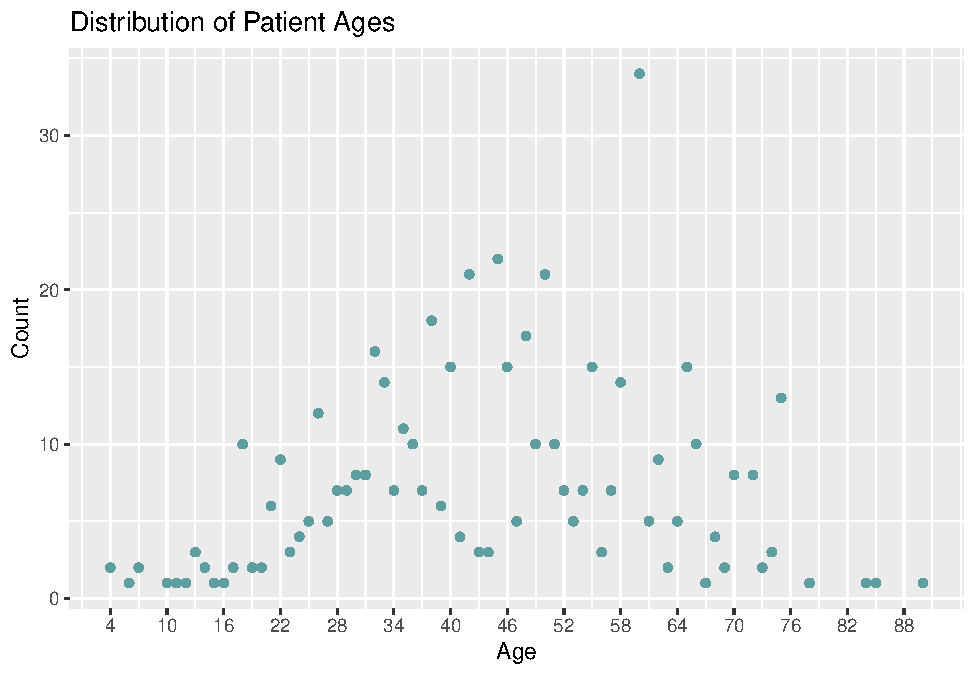
\includegraphics{LiverDisease_files/figure-latex/unnamed-chunk-9-1.pdf}
We breakdown the distribution of ages to the presence or absence of
liver disease. Again, we notice a good spread of age group for both
scenarios.

\begin{Shaded}
\begin{Highlighting}[]
\CommentTok{# Plotting distributions of ages based on liver diseases}
\NormalTok{training }\OperatorTok\StringTok{ }
\StringTok{  }\KeywordTok{ggplot}\NormalTok{(}\KeywordTok{aes}\NormalTok{(}\KeywordTok{as.numeric}\NormalTok{(}\KeywordTok{row.names}\NormalTok{(training)),Age, }\DataTypeTok{color=}\NormalTok{LiverDisease)) }\OperatorTok{+}
\StringTok{  }\KeywordTok{geom_point}\NormalTok{() }\OperatorTok{+}
\StringTok{  }\KeywordTok{labs}\NormalTok{(}\DataTypeTok{y=}\StringTok{"Age"}\NormalTok{, }\DataTypeTok{x =} \StringTok{"Number of patients"}\NormalTok{)}\OperatorTok{+}
\StringTok{  }\KeywordTok{facet_wrap}\NormalTok{( }\OperatorTok{~}\StringTok{ }\NormalTok{LiverDisease) }\OperatorTok{+}
\StringTok{  }\KeywordTok{ggtitle}\NormalTok{(}\StringTok{"Distribution of ages based on liver disease"}\NormalTok{)}
\end{Highlighting}
\end{Shaded}

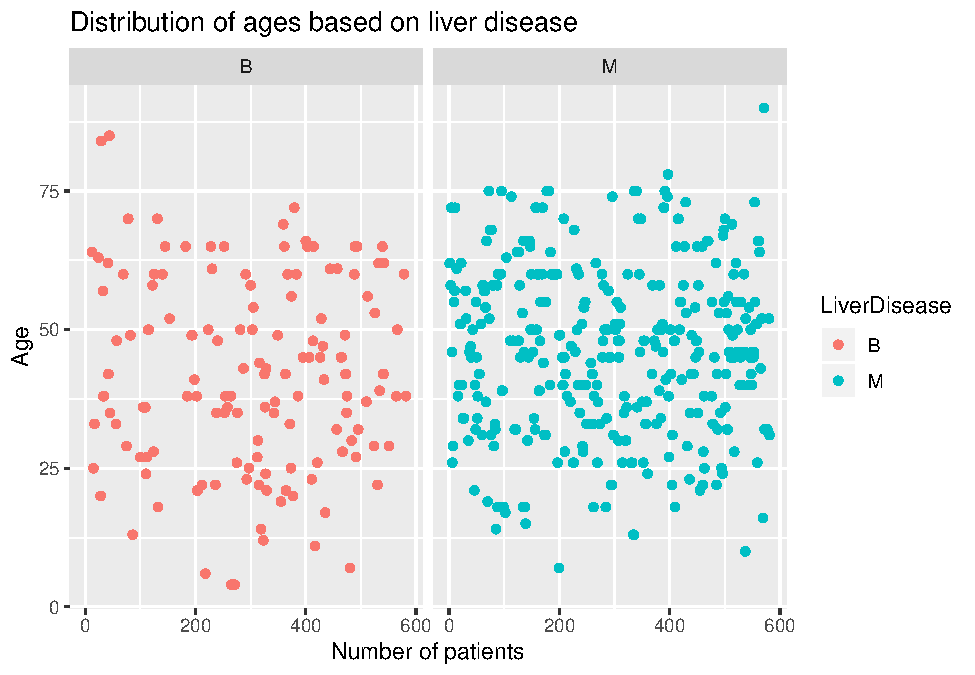
\includegraphics{LiverDisease_files/figure-latex/unnamed-chunk-10-1.pdf}

\subsection{Gender}

76\% of the patient records are of males. It would be good to have a
more and less equal distribution of records for both genders, although
we do not expect it to make any difference in our models.

\begin{Shaded}
\begin{Highlighting}[]
\CommentTok{# Getting summary of genders}
\KeywordTok{summary}\NormalTok{(training}\OperatorTok{$}\NormalTok{Gender)}
\end{Highlighting}
\end{Shaded}

\begin{verbatim}
## Female   Male 
##    125    398
\end{verbatim}

\textbackslash subsection\{Total\_Bilirubin and Direct\_Bilirubin\}
Bilirubin refers to any form of a yellowish pigment made in the liver
when red blood cells are broken down. The elevated levels indicate that
the liver is damaged. We find a similar trend with the variable that
Bilirubin levels are high for patients with liver diseases.

\begin{Shaded}
\begin{Highlighting}[]
\CommentTok{# Plotting distributions of Total_Bilirubin based on liver diseases}
\NormalTok{training }\OperatorTok\StringTok{ }
\StringTok{  }\KeywordTok{ggplot}\NormalTok{(}\KeywordTok{aes}\NormalTok{(}\KeywordTok{as.numeric}\NormalTok{(}\KeywordTok{row.names}\NormalTok{(training)),Total_Bilirubin, }\DataTypeTok{color=}\NormalTok{LiverDisease)) }\OperatorTok{+}
\StringTok{  }\KeywordTok{geom_boxplot}\NormalTok{() }\OperatorTok{+}
\StringTok{  }\KeywordTok{labs}\NormalTok{(}\DataTypeTok{y=}\StringTok{"Total_Bilirubin"}\NormalTok{, }\DataTypeTok{x =} \StringTok{"Number of patients"}\NormalTok{)}\OperatorTok{+}
\StringTok{  }\KeywordTok{facet_wrap}\NormalTok{( }\OperatorTok{~}\StringTok{ }\NormalTok{LiverDisease) }\OperatorTok{+}
\StringTok{  }\KeywordTok{ggtitle}\NormalTok{(}\StringTok{"Distribution of Total_Bilirubin based on liver disease"}\NormalTok{)}
\end{Highlighting}
\end{Shaded}

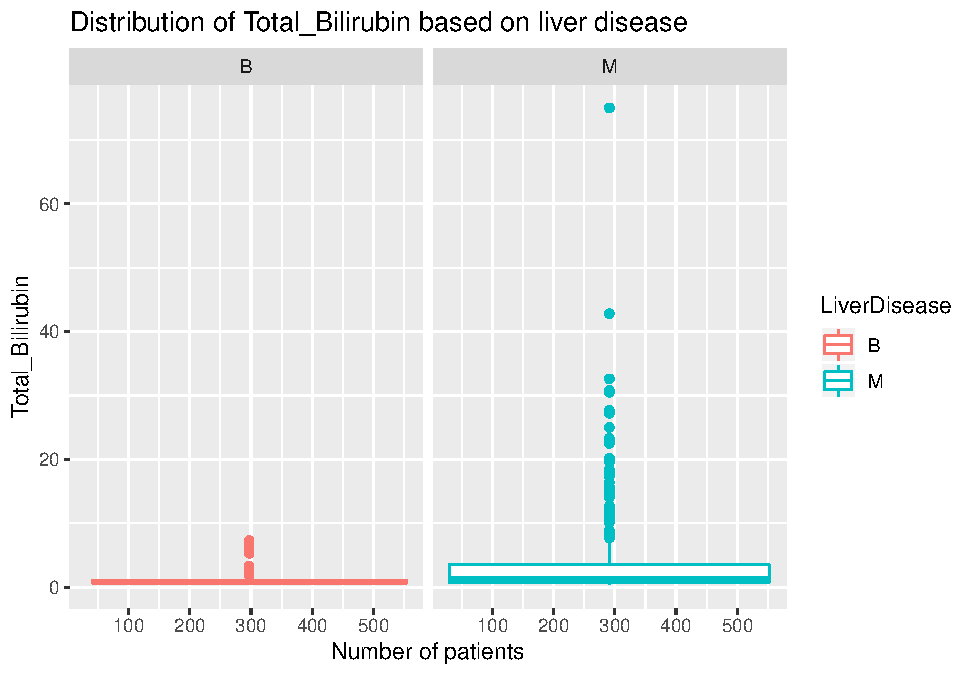
\includegraphics{LiverDisease_files/figure-latex/unnamed-chunk-12-1.pdf}

\begin{Shaded}
\begin{Highlighting}[]
\CommentTok{# Plotting distributions of Direct_Bilirubin based on liver disease}
\NormalTok{training }\OperatorTok\StringTok{ }
\StringTok{  }\KeywordTok{ggplot}\NormalTok{(}\KeywordTok{aes}\NormalTok{(}\KeywordTok{as.numeric}\NormalTok{(}\KeywordTok{row.names}\NormalTok{(training)),Direct_Bilirubin, }\DataTypeTok{color=}\NormalTok{LiverDisease)) }\OperatorTok{+}
\StringTok{  }\KeywordTok{geom_boxplot}\NormalTok{() }\OperatorTok{+}
\StringTok{  }\KeywordTok{labs}\NormalTok{(}\DataTypeTok{y=}\StringTok{"Direct_Bilirubin"}\NormalTok{, }\DataTypeTok{x =} \StringTok{"Number of patients"}\NormalTok{)}\OperatorTok{+}
\StringTok{  }\KeywordTok{facet_wrap}\NormalTok{( }\OperatorTok{~}\StringTok{ }\NormalTok{LiverDisease) }\OperatorTok{+}
\StringTok{  }\KeywordTok{ggtitle}\NormalTok{(}\StringTok{"Distribution of Direct_Bilirubin based on liver disease"}\NormalTok{)}
\end{Highlighting}
\end{Shaded}

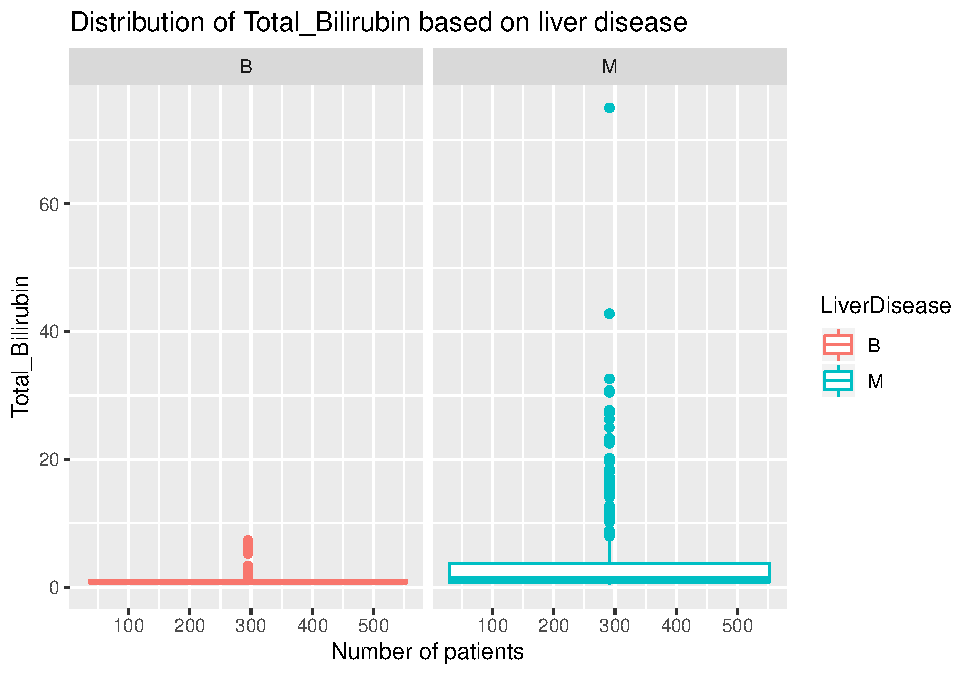
\includegraphics{LiverDisease_files/figure-latex/unnamed-chunk-13-1.pdf}

The correlations show that both bilirubins are weakly correlated with
liver disease. However, both bilirubins are highly correlated with each
other.

\begin{Shaded}
\begin{Highlighting}[]
\CommentTok{# Making a subset of data}
\NormalTok{subset_train <-}\StringTok{ }\NormalTok{training[}\KeywordTok{c}\NormalTok{(}\StringTok{"Total_Bilirubin"}\NormalTok{,}\StringTok{"Direct_Bilirubin"}\NormalTok{,}\StringTok{"LiverDisease"}\NormalTok{)]}
\CommentTok{# Converting disease variable to numeric format}
\NormalTok{subset_train <-}\StringTok{ }\KeywordTok{transform}\NormalTok{(subset_train, }\DataTypeTok{LiverDisease=} \KeywordTok{ifelse}\NormalTok{(subset_train}\OperatorTok{$}\NormalTok{LiverDisease}\OperatorTok{==}\StringTok{"M"}\NormalTok{, }\DecValTok{1}\NormalTok{,}\DecValTok{0}\NormalTok{))}
\CommentTok{# Looking at the coorelations}
\KeywordTok{cor}\NormalTok{(subset_train) }
\end{Highlighting}
\end{Shaded}

\begin{verbatim}
##                  Total_Bilirubin Direct_Bilirubin LiverDisease
## Total_Bilirubin        1.0000000        0.8584292    0.2065553
## Direct_Bilirubin       0.8584292        1.0000000    0.2347388
## LiverDisease           0.2065553        0.2347388    1.0000000
\end{verbatim}

\subsection{Alkaline Phosphotase}

Alkaline phosphatase (ALP) is an enzyme in a person's blood that helps
break down proteins. We notice that levels of ALP are comparatively high
for patients with liver diseases.

\begin{Shaded}
\begin{Highlighting}[]
\CommentTok{# Plotting distributions of Alkaline Phosphotase based on liver diseases}
\NormalTok{training }\OperatorTok\StringTok{ }
\StringTok{  }\KeywordTok{ggplot}\NormalTok{(}\KeywordTok{aes}\NormalTok{(}\KeywordTok{as.numeric}\NormalTok{(}\KeywordTok{row.names}\NormalTok{(training)),Alkaline_Phosphotase, }\DataTypeTok{color=}\NormalTok{LiverDisease)) }\OperatorTok{+}
\StringTok{  }\KeywordTok{geom_boxplot}\NormalTok{() }\OperatorTok{+}
\StringTok{  }\KeywordTok{labs}\NormalTok{(}\DataTypeTok{y=}\StringTok{"Alkaline Phosphotase"}\NormalTok{, }\DataTypeTok{x =} \StringTok{"Number of patients"}\NormalTok{)}\OperatorTok{+}
\StringTok{  }\KeywordTok{facet_wrap}\NormalTok{( }\OperatorTok{~}\StringTok{ }\NormalTok{LiverDisease) }\OperatorTok{+}
\StringTok{  }\KeywordTok{ggtitle}\NormalTok{(}\StringTok{"Distribution of Alkaline Phosphotase based on liver disease"}\NormalTok{)}
\end{Highlighting}
\end{Shaded}

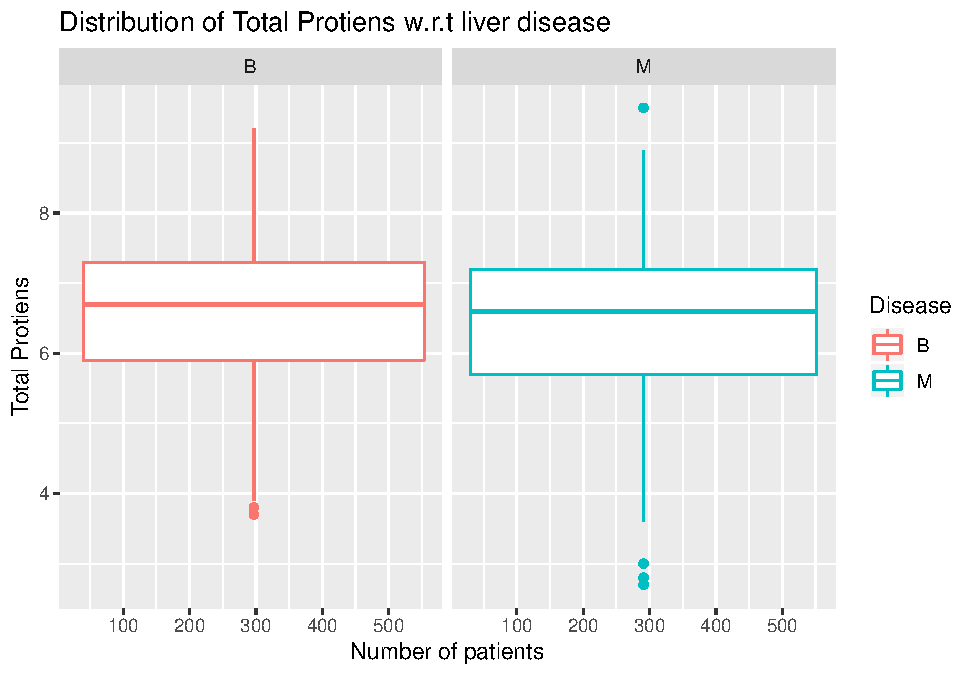
\includegraphics{LiverDisease_files/figure-latex/unnamed-chunk-15-1.pdf}

\textbackslash subsection\{Alamine\_Aminotransferase and
Aspartate\_Aminotransferase\} Aminotransferases are enzymes that are
important in the synthesis of amino acids, which form proteins. Alanine
aminotransferase (ALT) and Aspartate aminotransferase (AST) are found
primarily in the liver and kidney. High levels of ALT and AST are
expected for patients with liver diseases. We also observe the slightly
elevated levels of these enzymes for patients with liver diseases.

\begin{Shaded}
\begin{Highlighting}[]
\CommentTok{# Plotting distributions of Alamine Aminotransferase based on liver diseases}
\NormalTok{training }\OperatorTok\StringTok{ }
\StringTok{  }\KeywordTok{ggplot}\NormalTok{(}\KeywordTok{aes}\NormalTok{(}\KeywordTok{as.numeric}\NormalTok{(}\KeywordTok{row.names}\NormalTok{(training)),Alamine_Aminotransferase, }\DataTypeTok{color=}\NormalTok{LiverDisease)) }\OperatorTok{+}
\StringTok{  }\KeywordTok{geom_boxplot}\NormalTok{() }\OperatorTok{+}
\StringTok{  }\KeywordTok{labs}\NormalTok{(}\DataTypeTok{y=}\StringTok{"Alamine Aminotransferase"}\NormalTok{, }\DataTypeTok{x =} \StringTok{"Number of patients"}\NormalTok{)}\OperatorTok{+}
\StringTok{  }\KeywordTok{facet_wrap}\NormalTok{( }\OperatorTok{~}\StringTok{ }\NormalTok{LiverDisease) }\OperatorTok{+}
\StringTok{  }\KeywordTok{ggtitle}\NormalTok{(}\StringTok{"Distribution of Alamine Aminotransferase based on liver disease"}\NormalTok{) }
\end{Highlighting}
\end{Shaded}

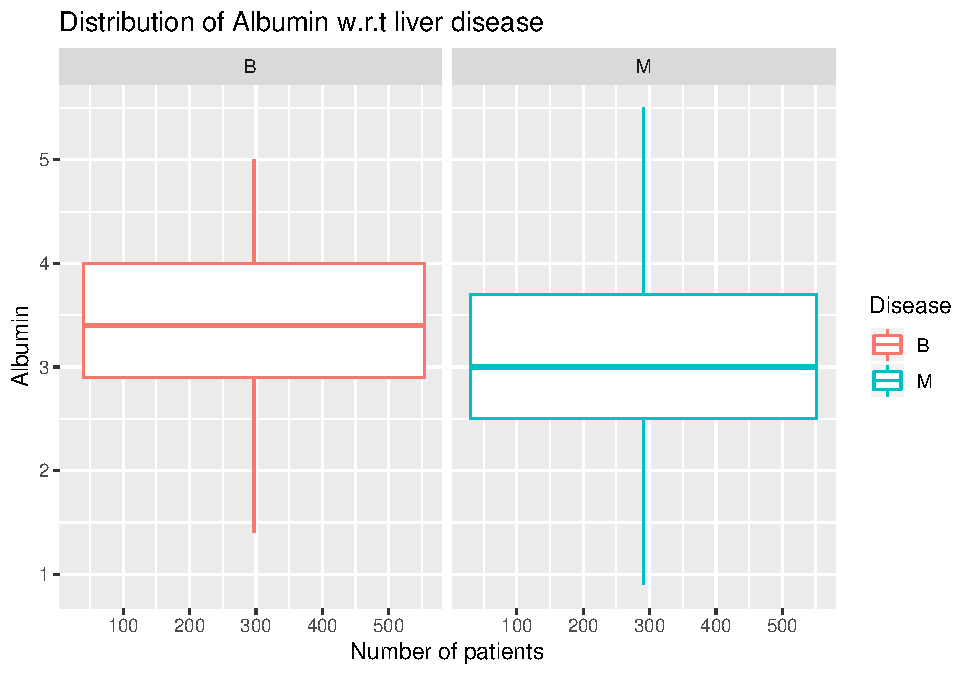
\includegraphics{LiverDisease_files/figure-latex/unnamed-chunk-16-1.pdf}

\begin{Shaded}
\begin{Highlighting}[]
\CommentTok{# Plotting distributions of Aspartate_Aminotransferase based on liver diseases}
\NormalTok{training }\OperatorTok\StringTok{ }
\StringTok{  }\KeywordTok{ggplot}\NormalTok{(}\KeywordTok{aes}\NormalTok{(}\KeywordTok{as.numeric}\NormalTok{(}\KeywordTok{row.names}\NormalTok{(training)),Aspartate_Aminotransferase, }\DataTypeTok{color=}\NormalTok{LiverDisease)) }\OperatorTok{+}
\StringTok{  }\KeywordTok{geom_boxplot}\NormalTok{() }\OperatorTok{+}
\StringTok{  }\KeywordTok{labs}\NormalTok{(}\DataTypeTok{y=}\StringTok{"Aspartate Aminotransferase"}\NormalTok{, }\DataTypeTok{x =} \StringTok{"Number of patients"}\NormalTok{)}\OperatorTok{+}
\StringTok{  }\KeywordTok{facet_wrap}\NormalTok{( }\OperatorTok{~}\StringTok{ }\NormalTok{LiverDisease) }\OperatorTok{+}
\StringTok{  }\KeywordTok{ggtitle}\NormalTok{(}\StringTok{"Distribution of Aspartate Aminotransferase based on liver disease"}\NormalTok{) }
\end{Highlighting}
\end{Shaded}

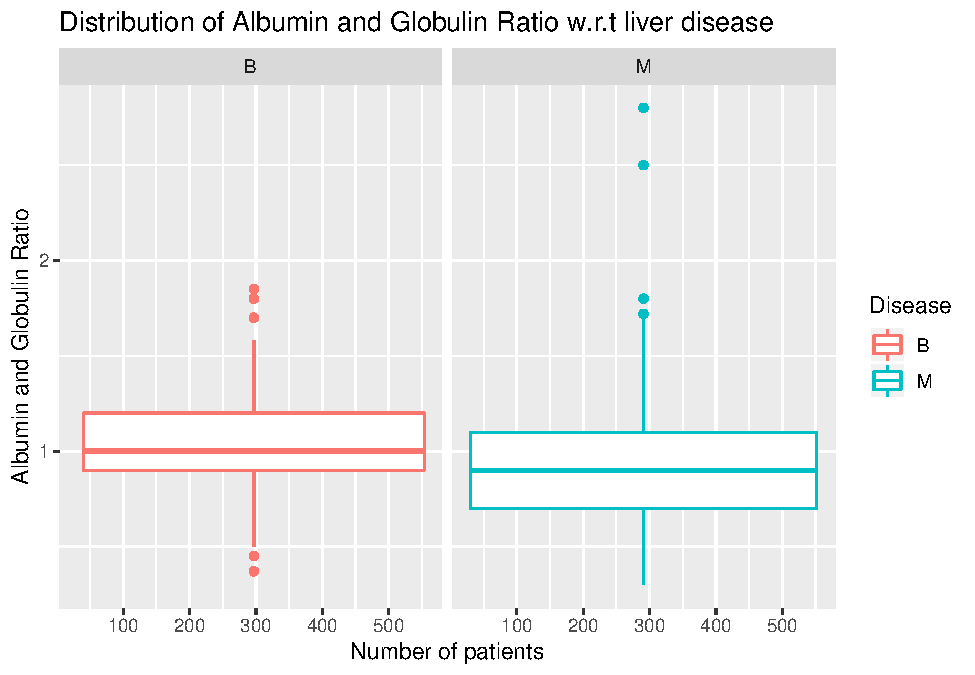
\includegraphics{LiverDisease_files/figure-latex/unnamed-chunk-17-1.pdf}

Contrary to bilirubins, there exists a weak correlation between both
aminotransferases.

\begin{Shaded}
\begin{Highlighting}[]
\CommentTok{# Making a subset of data}
\NormalTok{subset_train <-}\StringTok{ }\NormalTok{training[}\KeywordTok{c}\NormalTok{(}\StringTok{"Alkaline_Phosphotase"}\NormalTok{,}\StringTok{"Aspartate_Aminotransferase"}\NormalTok{,}\StringTok{"LiverDisease"}\NormalTok{)]}

\CommentTok{# Converting disease variable to numeric format}
\NormalTok{subset_train <-}\StringTok{ }\KeywordTok{transform}\NormalTok{(subset_train, }\DataTypeTok{LiverDisease=} \KeywordTok{ifelse}\NormalTok{(subset_train}\OperatorTok{$}\NormalTok{LiverDisease}\OperatorTok{==}\StringTok{"M"}\NormalTok{, }\DecValTok{1}\NormalTok{,}\DecValTok{0}\NormalTok{))}

\CommentTok{# Looking at the coorelations}
\KeywordTok{cor}\NormalTok{(subset_train) }
\end{Highlighting}
\end{Shaded}

\begin{verbatim}
##                            Alkaline_Phosphotase Aspartate_Aminotransferase
## Alkaline_Phosphotase                   1.000000                  0.2156400
## Aspartate_Aminotransferase             0.215640                  1.0000000
## LiverDisease                           0.178212                  0.1488358
##                            LiverDisease
## Alkaline_Phosphotase          0.1782120
## Aspartate_Aminotransferase    0.1488358
## LiverDisease                  1.0000000
\end{verbatim}

\subsection{Total Protiens}

The total protein test measures the total amount of protein in your
body. The distributions indicate that we can diagnose liver disease
reliably using this variable.

\begin{Shaded}
\begin{Highlighting}[]
\CommentTok{# Plotting distributions of Total Protiens based on liver diseases}
\NormalTok{training }\OperatorTok\StringTok{ }
\StringTok{  }\KeywordTok{ggplot}\NormalTok{(}\KeywordTok{aes}\NormalTok{(}\KeywordTok{as.numeric}\NormalTok{(}\KeywordTok{row.names}\NormalTok{(training)),Total_Protiens, }\DataTypeTok{color=}\NormalTok{LiverDisease)) }\OperatorTok{+}
\StringTok{  }\KeywordTok{geom_boxplot}\NormalTok{() }\OperatorTok{+}
\StringTok{  }\KeywordTok{labs}\NormalTok{(}\DataTypeTok{y=}\StringTok{"Total Protiens"}\NormalTok{, }\DataTypeTok{x =} \StringTok{"Number of patients"}\NormalTok{)}\OperatorTok{+}
\StringTok{  }\KeywordTok{facet_wrap}\NormalTok{( }\OperatorTok{~}\StringTok{ }\NormalTok{LiverDisease) }\OperatorTok{+}
\StringTok{  }\KeywordTok{ggtitle}\NormalTok{(}\StringTok{"Distribution of Total Protiens based on liver diseases"}\NormalTok{) }
\end{Highlighting}
\end{Shaded}

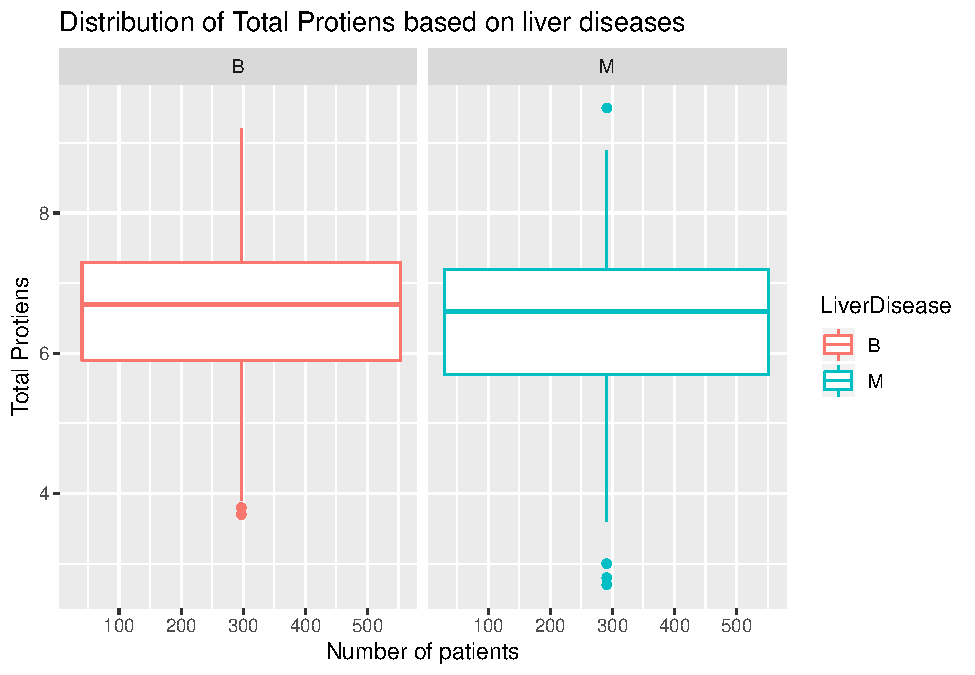
\includegraphics{LiverDisease_files/figure-latex/unnamed-chunk-19-1.pdf}

\subsection{Albumin}

Albumin is a protein made by the liver to keep fluid in the bloodstream.
The low levels of albumin often indicate a problem with the liver, and
we notice a similar trend with this variable.

\begin{Shaded}
\begin{Highlighting}[]
\CommentTok{# Plotting distributions of Albumin based on liver diseases}
\NormalTok{training }\OperatorTok\StringTok{ }
\StringTok{  }\KeywordTok{ggplot}\NormalTok{(}\KeywordTok{aes}\NormalTok{(}\KeywordTok{as.numeric}\NormalTok{(}\KeywordTok{row.names}\NormalTok{(training)),Albumin, }\DataTypeTok{color=}\NormalTok{LiverDisease)) }\OperatorTok{+}
\StringTok{  }\KeywordTok{geom_boxplot}\NormalTok{() }\OperatorTok{+}
\StringTok{  }\KeywordTok{labs}\NormalTok{(}\DataTypeTok{y=}\StringTok{"Albumin"}\NormalTok{, }\DataTypeTok{x =} \StringTok{"Number of patients"}\NormalTok{)}\OperatorTok{+}
\StringTok{  }\KeywordTok{facet_wrap}\NormalTok{( }\OperatorTok{~}\StringTok{ }\NormalTok{LiverDisease) }\OperatorTok{+}
\StringTok{  }\KeywordTok{ggtitle}\NormalTok{(}\StringTok{"Distribution of Albumin based on liver disease"}\NormalTok{) }
\end{Highlighting}
\end{Shaded}

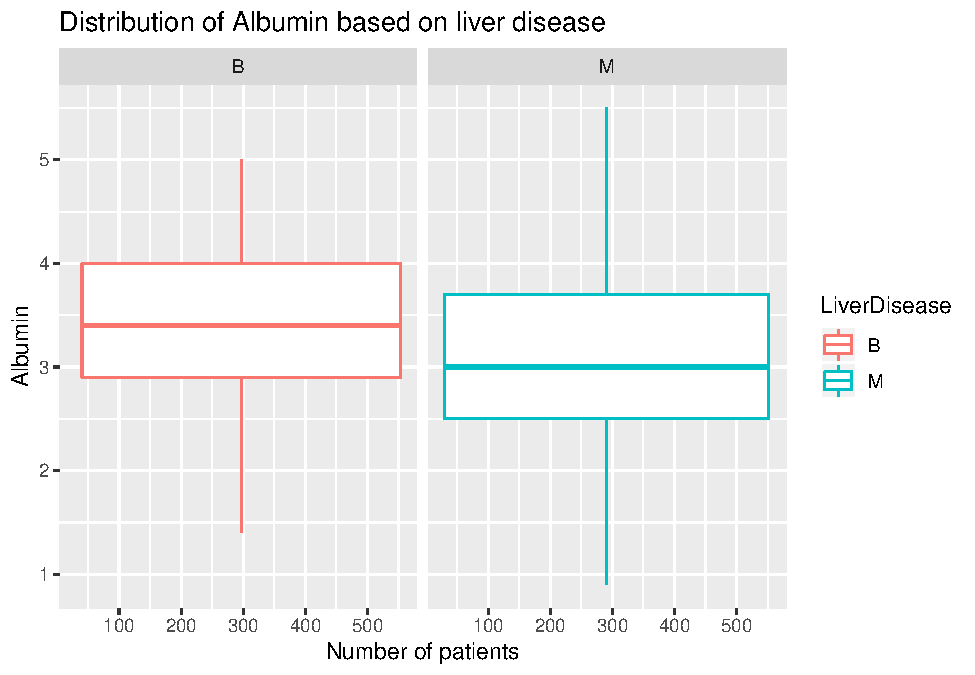
\includegraphics{LiverDisease_files/figure-latex/unnamed-chunk-20-1.pdf}

\textbackslash subsection\{Albumin\_and\_Globulin\_Ratio\} These
proteins are crucial for body growth, development, and health. They form
the structural part of most organs and makeup enzymes and hormones that
regulate body functions. The low ratios refer to liver issues, and we
can notice the same from distributions graphs.

\begin{Shaded}
\begin{Highlighting}[]
\CommentTok{# Plotting distributions of Albumin based on liver diseases}
\NormalTok{training }\OperatorTok\StringTok{ }
\StringTok{  }\KeywordTok{ggplot}\NormalTok{(}\KeywordTok{aes}\NormalTok{(}\KeywordTok{as.numeric}\NormalTok{(}\KeywordTok{row.names}\NormalTok{(training)),Albumin_and_Globulin_Ratio, }\DataTypeTok{color=}\NormalTok{LiverDisease)) }\OperatorTok{+}
\StringTok{  }\KeywordTok{geom_boxplot}\NormalTok{() }\OperatorTok{+}
\StringTok{  }\KeywordTok{labs}\NormalTok{(}\DataTypeTok{y=}\StringTok{"Albumin and Globulin Ratio"}\NormalTok{, }\DataTypeTok{x =} \StringTok{"Number of patients"}\NormalTok{)}\OperatorTok{+}
\StringTok{  }\KeywordTok{facet_wrap}\NormalTok{( }\OperatorTok{~}\StringTok{ }\NormalTok{LiverDisease) }\OperatorTok{+}
\StringTok{  }\KeywordTok{ggtitle}\NormalTok{(}\StringTok{"Distribution of Albumin and Globulin Ratio based on liver disease"}\NormalTok{) }
\end{Highlighting}
\end{Shaded}

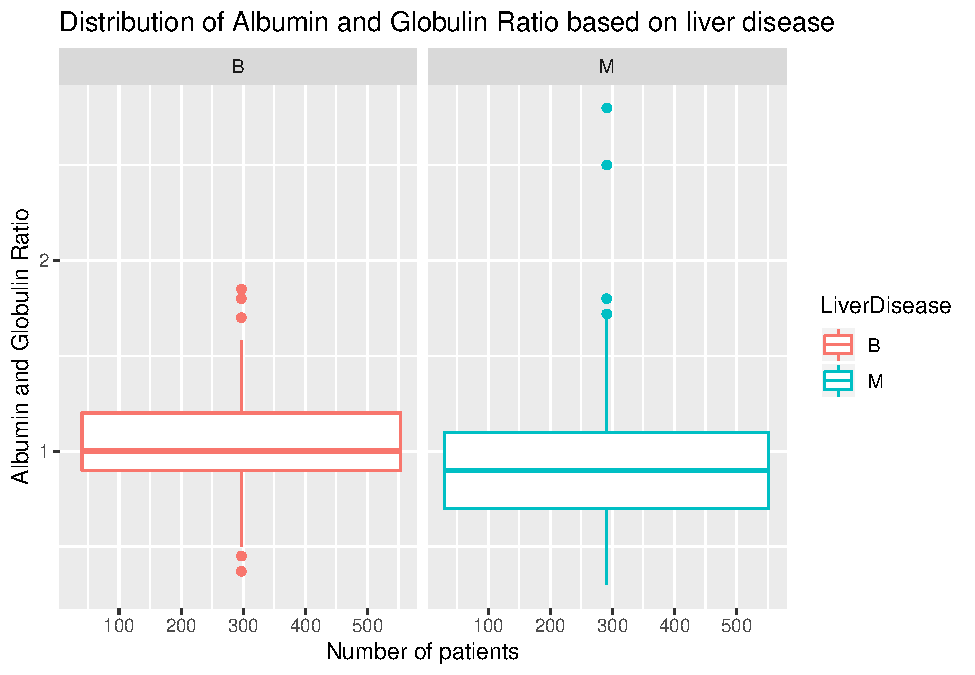
\includegraphics{LiverDisease_files/figure-latex/unnamed-chunk-21-1.pdf}

\section{Methods}
\label{sec:methods}

Based on the discussion in Section \ref{sec:dataanalysis}, we will not
use ``Age'' and ``Total Protein'' variables to train the machine
learning models. We remove these variables from both training and
validation datasets.

\begin{Shaded}
\begin{Highlighting}[]
\CommentTok{# Deleting the column 'Dataset' as no longer required}
\NormalTok{training<-}\KeywordTok{within}\NormalTok{(training, }\KeywordTok{rm}\NormalTok{(Age,Total_Protiens))}
\NormalTok{validation<-}\KeywordTok{within}\NormalTok{(validation, }\KeywordTok{rm}\NormalTok{(Age,Total_Protiens))}
\end{Highlighting}
\end{Shaded}

\subsection{Logistic Regression}

We use logistic regression with cross-validation of 10 folds to train
the model.

\begin{Shaded}
\begin{Highlighting}[]
\CommentTok{# Defining a cross-validation (10 K folds )}
\NormalTok{control <-}\StringTok{ }\KeywordTok{trainControl}\NormalTok{(}\DataTypeTok{method =} \StringTok{"cv"}\NormalTok{, }\DataTypeTok{number =}\DecValTok{10}\NormalTok{)}

\CommentTok{# Train logistic regression model}
\NormalTok{train_glm <-}\StringTok{ }\KeywordTok{train}\NormalTok{(LiverDisease }\OperatorTok{~}\NormalTok{., }
                   \DataTypeTok{method =} \StringTok{"glm"}\NormalTok{,}
                   \DataTypeTok{data =}\NormalTok{ training,}
                   \DataTypeTok{trControl=}\NormalTok{control)}
\end{Highlighting}
\end{Shaded}

\begin{verbatim}
## Warning: glm.fit: fitted probabilities numerically 0 or 1 occurred

## Warning: glm.fit: fitted probabilities numerically 0 or 1 occurred

## Warning: glm.fit: fitted probabilities numerically 0 or 1 occurred

## Warning: glm.fit: fitted probabilities numerically 0 or 1 occurred

## Warning: glm.fit: fitted probabilities numerically 0 or 1 occurred

## Warning: glm.fit: fitted probabilities numerically 0 or 1 occurred

## Warning: glm.fit: fitted probabilities numerically 0 or 1 occurred
\end{verbatim}

\begin{Shaded}
\begin{Highlighting}[]
\KeywordTok{sprintf}\NormalTok{(}\StringTok{"The accuracy of GLM = %f"}\NormalTok{,train_glm}\OperatorTok{$}\NormalTok{results}\OperatorTok{$}\NormalTok{Accuracy)}
\end{Highlighting}
\end{Shaded}

\begin{verbatim}
## [1] "The accuracy of GLM = 0.703512"
\end{verbatim}

\begin{Shaded}
\begin{Highlighting}[]
\NormalTok{model_results <-}\StringTok{ }\KeywordTok{data_frame}\NormalTok{(}\DataTypeTok{method =} \StringTok{"glm"}\NormalTok{, }\DataTypeTok{Accuracy =}\NormalTok{ train_glm}\OperatorTok{$}\NormalTok{results}\OperatorTok{$}\NormalTok{Accuracy)}
\end{Highlighting}
\end{Shaded}

\begin{verbatim}
## Warning: `data_frame()` is deprecated, use `tibble()`.
## This warning is displayed once per session.
\end{verbatim}

\subsection{K-nearest neigbors (knn)}

We use knn with cross-validation of 10 folds to train the model.

\begin{Shaded}
\begin{Highlighting}[]
\CommentTok{# Defining a cross validation (10 K folds )}
\NormalTok{control <-}\StringTok{ }\KeywordTok{trainControl}\NormalTok{(}\DataTypeTok{method =} \StringTok{"cv"}\NormalTok{, }\DataTypeTok{number =} \DecValTok{10}\NormalTok{)}
\CommentTok{# Train knn model}
\NormalTok{train_knn <-}\StringTok{ }\KeywordTok{train}\NormalTok{(LiverDisease}\OperatorTok{~}\StringTok{ }\NormalTok{.,}
                   \DataTypeTok{method =} \StringTok{"knn"}\NormalTok{, }
                   \DataTypeTok{data =}\NormalTok{ training,}
                   \DataTypeTok{tuneGrid =} \KeywordTok{data.frame}\NormalTok{(}\DataTypeTok{k =} \KeywordTok{seq}\NormalTok{(}\DecValTok{3}\NormalTok{, }\DecValTok{51}\NormalTok{, }\DecValTok{2}\NormalTok{)),}
                   \DataTypeTok{trControl =}\NormalTok{ control)}

\KeywordTok{ggplot}\NormalTok{(train_knn, }\DataTypeTok{highlight =} \OtherTok{TRUE}\NormalTok{)}
\end{Highlighting}
\end{Shaded}

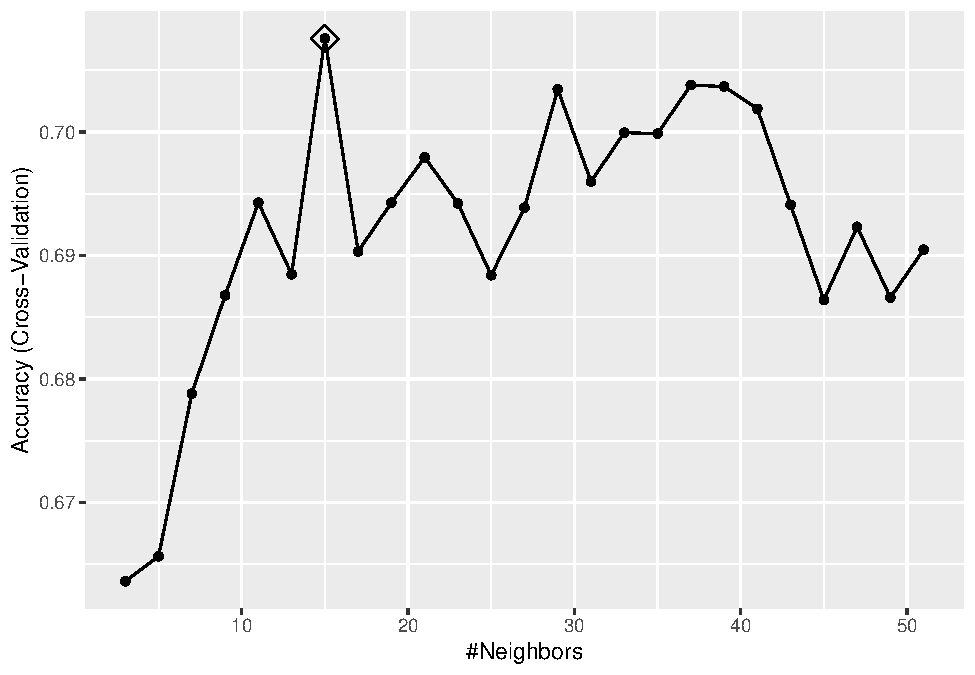
\includegraphics{LiverDisease_files/figure-latex/unnamed-chunk-24-1.pdf}

\begin{Shaded}
\begin{Highlighting}[]
\KeywordTok{sprintf}\NormalTok{(}\StringTok{"The best accuracy = %f"}\NormalTok{,}\KeywordTok{max}\NormalTok{(train_knn}\OperatorTok{$}\NormalTok{results}\OperatorTok{$}\NormalTok{Accuracy))}
\end{Highlighting}
\end{Shaded}

\begin{verbatim}
## [1] "The best accuracy = 0.707565"
\end{verbatim}

\begin{Shaded}
\begin{Highlighting}[]
\CommentTok{# Stroing the results}
\NormalTok{model_results <-}\StringTok{ }\KeywordTok{bind_rows}\NormalTok{(model_results,}\KeywordTok{data_frame}\NormalTok{(}\DataTypeTok{method=}\StringTok{"knn"}\NormalTok{,  }
                                     \DataTypeTok{Accuracy =} \KeywordTok{max}\NormalTok{(train_knn}\OperatorTok{$}\NormalTok{results}\OperatorTok{$}\NormalTok{Accuracy) ))}
\end{Highlighting}
\end{Shaded}

\subsection{Partial Least Squares (PLS)}

We use PLS with cross-validation of 10 folds to train the model.

\begin{Shaded}
\begin{Highlighting}[]
\KeywordTok{set.seed}\NormalTok{(}\DecValTok{10}\NormalTok{)}
\CommentTok{# Defining a cross validation (10 K folds )}
\NormalTok{control <-}\StringTok{ }\KeywordTok{trainControl}\NormalTok{(}\DataTypeTok{method =} \StringTok{"cv"}\NormalTok{, }\DataTypeTok{number =} \DecValTok{10}\NormalTok{)}
\CommentTok{# Train the model}
\NormalTok{train_pls <-}\StringTok{ }\KeywordTok{train}\NormalTok{(LiverDisease}\OperatorTok{~}\NormalTok{.,}
                   \DataTypeTok{method =} \StringTok{"pls"}\NormalTok{,}
                   \DataTypeTok{data =}\NormalTok{ training,}
                   \DataTypeTok{preProc =} \KeywordTok{c}\NormalTok{(}\StringTok{"center"}\NormalTok{, }\StringTok{"scale"}\NormalTok{),}
                   \DataTypeTok{tuneLength =} \DecValTok{15}\NormalTok{,}
                   \DataTypeTok{trControl =}\NormalTok{ control)}

\KeywordTok{sprintf}\NormalTok{(}\StringTok{"The accuracy of PLS  = %f"}\NormalTok{,}\KeywordTok{max}\NormalTok{(train_pls}\OperatorTok{$}\NormalTok{results}\OperatorTok{$}\NormalTok{Accuracy))}
\end{Highlighting}
\end{Shaded}

\begin{verbatim}
## [1] "The accuracy of PLS  = 0.720860"
\end{verbatim}

\begin{Shaded}
\begin{Highlighting}[]
\CommentTok{# Stroing the results}
\NormalTok{model_results <-}\StringTok{ }\KeywordTok{bind_rows}\NormalTok{(model_results,}\KeywordTok{data_frame}\NormalTok{(}\DataTypeTok{method=}\StringTok{"pls"}\NormalTok{,  }
                                     \DataTypeTok{Accuracy =} \KeywordTok{max}\NormalTok{(train_pls}\OperatorTok{$}\NormalTok{results}\OperatorTok{$}\NormalTok{Accuracy) ))}
\end{Highlighting}
\end{Shaded}

\subsection{Linear Discriminant Analysis (LDA)}

The LDA is a statistical classifier, and we use it with a
cross-validation of 10 folds for training.

\begin{Shaded}
\begin{Highlighting}[]
\CommentTok{# Defining a cross validation (10 K folds )}
\NormalTok{control <-}\StringTok{ }\KeywordTok{trainControl}\NormalTok{(}\DataTypeTok{method =} \StringTok{"cv"}\NormalTok{, }\DataTypeTok{number=}\DecValTok{10}\NormalTok{)}
\CommentTok{# Train the model}
\NormalTok{train_lda <-}\StringTok{ }\KeywordTok{train}\NormalTok{(LiverDisease}\OperatorTok{~}\NormalTok{., }
                   \DataTypeTok{method =} \StringTok{"lda"}\NormalTok{,}
                   \DataTypeTok{data =}\NormalTok{ training,}
                   \DataTypeTok{trControl =}\NormalTok{ control)}

\KeywordTok{sprintf}\NormalTok{(}\StringTok{"The accuracy of lda = %f"}\NormalTok{,}\KeywordTok{max}\NormalTok{(train_lda}\OperatorTok{$}\NormalTok{results}\OperatorTok{$}\NormalTok{Accuracy))}
\end{Highlighting}
\end{Shaded}

\begin{verbatim}
## [1] "The accuracy of lda = 0.717124"
\end{verbatim}

\begin{Shaded}
\begin{Highlighting}[]
\CommentTok{# Stroing the results}
\NormalTok{model_results <-}\StringTok{ }\KeywordTok{bind_rows}\NormalTok{(model_results,}\KeywordTok{data_frame}\NormalTok{(}\DataTypeTok{method=}\StringTok{"lda"}\NormalTok{,  }
                                     \DataTypeTok{Accuracy =} \KeywordTok{max}\NormalTok{(train_lda}\OperatorTok{$}\NormalTok{results}\OperatorTok{$}\NormalTok{Accuracy) ))}
\end{Highlighting}
\end{Shaded}

\subsection{Quadratic Discriminant Analysis (QDA)}

The QDA is a statistical classifier, and we use it with a
cross-validation of 10 folds for training.

\begin{Shaded}
\begin{Highlighting}[]
\CommentTok{# Defining a cross validation (10 K folds )}
\NormalTok{control <-}\StringTok{ }\KeywordTok{trainControl}\NormalTok{(}\DataTypeTok{method =} \StringTok{"cv"}\NormalTok{, }\DataTypeTok{number=}\DecValTok{10}\NormalTok{)}
\CommentTok{# Train the model}
\NormalTok{train_qda <-}\StringTok{ }\KeywordTok{train}\NormalTok{(LiverDisease}\OperatorTok{~}\NormalTok{.,}
                   \DataTypeTok{method =} \StringTok{"qda"}\NormalTok{,}
                   \DataTypeTok{data =}\NormalTok{ training,}
                   \DataTypeTok{trControl =}\NormalTok{ control)}

\KeywordTok{sprintf}\NormalTok{(}\StringTok{"The accuracy of qda = %f"}\NormalTok{,}\KeywordTok{max}\NormalTok{(train_qda}\OperatorTok{$}\NormalTok{results}\OperatorTok{$}\NormalTok{Accuracy))}
\end{Highlighting}
\end{Shaded}

\begin{verbatim}
## [1] "The accuracy of qda = 0.539227"
\end{verbatim}

\begin{Shaded}
\begin{Highlighting}[]
\CommentTok{# Stroing the results}
\NormalTok{model_results <-}\StringTok{ }\KeywordTok{bind_rows}\NormalTok{(model_results,}\KeywordTok{data_frame}\NormalTok{(}\DataTypeTok{method=}\StringTok{"qda"}\NormalTok{,  }
                                     \DataTypeTok{Accuracy =} \KeywordTok{max}\NormalTok{(train_qda}\OperatorTok{$}\NormalTok{results}\OperatorTok{$}\NormalTok{Accuracy) ))}
\end{Highlighting}
\end{Shaded}

\subsection{Decision Tress}

We use decision trees with a cross-validation of 10 folds for training.

\begin{Shaded}
\begin{Highlighting}[]
\CommentTok{# Defining a cross validation (10 K folds )}
\NormalTok{control <-}\StringTok{ }\KeywordTok{trainControl}\NormalTok{(}\DataTypeTok{method =} \StringTok{"cv"}\NormalTok{, }\DataTypeTok{number =} \DecValTok{10}\NormalTok{)}
\CommentTok{# Train the model}
\NormalTok{train_rpart <-}\StringTok{ }\KeywordTok{train}\NormalTok{(LiverDisease}\OperatorTok{~}\NormalTok{., }
                     \DataTypeTok{method =} \StringTok{"rpart"}\NormalTok{,}
                     \DataTypeTok{data =}\NormalTok{ training,}
                     \DataTypeTok{trControl =}\NormalTok{ control,}
                     \DataTypeTok{tuneGrid =} \KeywordTok{data.frame}\NormalTok{(}\DataTypeTok{cp =} \KeywordTok{seq}\NormalTok{(}\DecValTok{0}\NormalTok{, }\FloatTok{0.05}\NormalTok{, }\DataTypeTok{len =} \DecValTok{25}\NormalTok{)))}
\KeywordTok{ggplot}\NormalTok{(train_rpart)}
\end{Highlighting}
\end{Shaded}

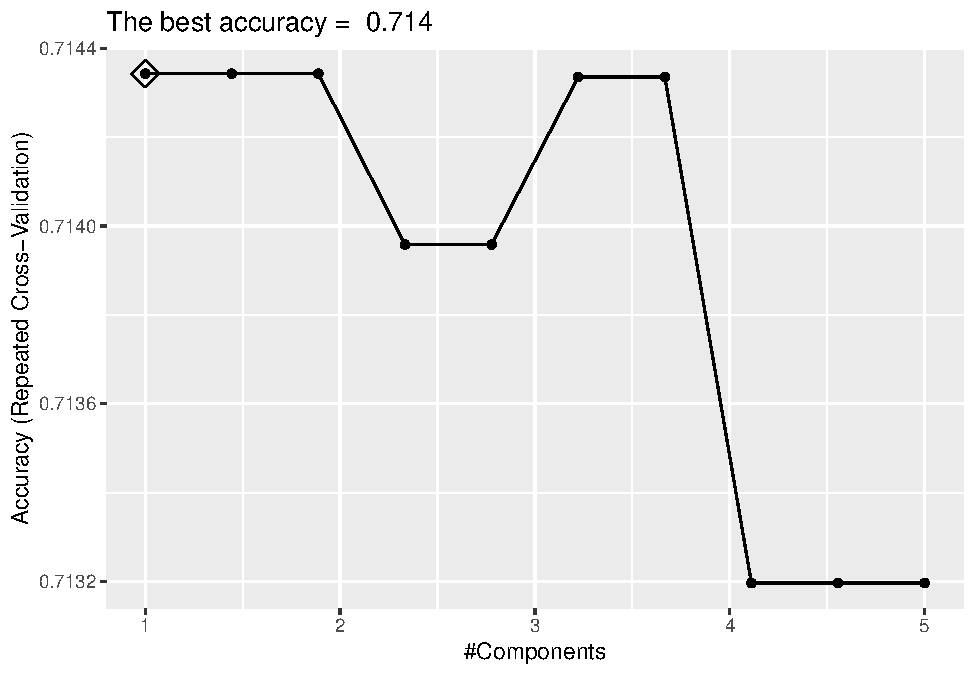
\includegraphics{LiverDisease_files/figure-latex/unnamed-chunk-28-1.pdf}

\begin{Shaded}
\begin{Highlighting}[]
\KeywordTok{sprintf}\NormalTok{(}\StringTok{"The accuracy of decision tree = %f"}\NormalTok{,}\KeywordTok{max}\NormalTok{(train_rpart}\OperatorTok{$}\NormalTok{results}\OperatorTok{$}\NormalTok{Accuracy))}
\end{Highlighting}
\end{Shaded}

\begin{verbatim}
## [1] "The accuracy of decision tree = 0.724688"
\end{verbatim}

\begin{Shaded}
\begin{Highlighting}[]
\CommentTok{# Stroing the results}
\NormalTok{model_results <-}\StringTok{ }\KeywordTok{bind_rows}\NormalTok{(model_results,}\KeywordTok{data_frame}\NormalTok{(}\DataTypeTok{method=}\StringTok{"rpart"}\NormalTok{,  }
                                     \DataTypeTok{Accuracy =} \KeywordTok{max}\NormalTok{(train_rpart}\OperatorTok{$}\NormalTok{results}\OperatorTok{$}\NormalTok{Accuracy) ))}
\end{Highlighting}
\end{Shaded}

\subsection{Random Forests}

We use random forests with a cross-validation of 10 folds for training.

\begin{Shaded}
\begin{Highlighting}[]
\CommentTok{# Defining a cross validation (10 K folds )}
\NormalTok{control <-}\StringTok{ }\KeywordTok{trainControl}\NormalTok{(}\DataTypeTok{method =} \StringTok{"cv"}\NormalTok{, }\DataTypeTok{number =} \DecValTok{10}\NormalTok{)}
\CommentTok{# Train the model}
\NormalTok{train_rf <-}\StringTok{ }\KeywordTok{train}\NormalTok{(LiverDisease}\OperatorTok{~}\NormalTok{.,}
                     \DataTypeTok{method =} \StringTok{"rf"}\NormalTok{,}
                     \DataTypeTok{data =}\NormalTok{ training,}
                     \DataTypeTok{trControl =}\NormalTok{ control,}
                     \DataTypeTok{tuneGrid =} \KeywordTok{data.frame}\NormalTok{(}\DataTypeTok{mtry=}\KeywordTok{seq}\NormalTok{(}\DecValTok{1}\NormalTok{,}\DecValTok{7}\NormalTok{)),}
                     \DataTypeTok{ntree=}\DecValTok{100}\NormalTok{)}
\KeywordTok{sprintf}\NormalTok{(}\StringTok{"The accuracy of forest tree = %f"}\NormalTok{,}\KeywordTok{max}\NormalTok{(train_rf}\OperatorTok{$}\NormalTok{results}\OperatorTok{$}\NormalTok{Accuracy))}
\end{Highlighting}
\end{Shaded}

\begin{verbatim}
## [1] "The accuracy of forest tree = 0.728628"
\end{verbatim}

\begin{Shaded}
\begin{Highlighting}[]
\CommentTok{# Stroing the results}
\NormalTok{model_results <-}\StringTok{ }\KeywordTok{bind_rows}\NormalTok{(model_results,}\KeywordTok{data_frame}\NormalTok{(}\DataTypeTok{method=}\StringTok{"rf"}\NormalTok{,  }
                                     \DataTypeTok{Accuracy =} \KeywordTok{max}\NormalTok{(train_rf}\OperatorTok{$}\NormalTok{results}\OperatorTok{$}\NormalTok{Accuracy) ))}
\end{Highlighting}
\end{Shaded}

\subsection{Support Vector Machine}

We use support vector machine with a cross-validation of 10 folds for
training.

\begin{Shaded}
\begin{Highlighting}[]
\CommentTok{# Defining a cross validation (10 K folds )}
\NormalTok{control <-}\StringTok{ }\KeywordTok{trainControl}\NormalTok{(}\DataTypeTok{method =} \StringTok{"cv"}\NormalTok{, }\DataTypeTok{number =} \DecValTok{10}\NormalTok{)}
\CommentTok{# Train the model}
\NormalTok{train_svm <-}\StringTok{ }\KeywordTok{train}\NormalTok{(LiverDisease}\OperatorTok{~}\NormalTok{.,}
                   \DataTypeTok{data =}\NormalTok{ training,}
                   \DataTypeTok{method =} \StringTok{"svmLinear"}\NormalTok{,}
                   \DataTypeTok{trControl =}\NormalTok{ control)}

\KeywordTok{sprintf}\NormalTok{(}\StringTok{"The accuracy of svm = %f"}\NormalTok{,}\KeywordTok{max}\NormalTok{(train_svm}\OperatorTok{$}\NormalTok{results}\OperatorTok{$}\NormalTok{Accuracy))}
\end{Highlighting}
\end{Shaded}

\begin{verbatim}
## [1] "The accuracy of svm = 0.718973"
\end{verbatim}

\begin{Shaded}
\begin{Highlighting}[]
\CommentTok{# Stroing the results}
\NormalTok{model_results <-}\StringTok{ }\KeywordTok{bind_rows}\NormalTok{(model_results,}\KeywordTok{data_frame}\NormalTok{(}\DataTypeTok{method=}\StringTok{"svm"}\NormalTok{,  }
                                     \DataTypeTok{Accuracy =} \KeywordTok{max}\NormalTok{(train_svm}\OperatorTok{$}\NormalTok{results}\OperatorTok{$}\NormalTok{Accuracy) ))}
\end{Highlighting}
\end{Shaded}

\subsection{Adaptive Boosting (Adaboost)}

AdaBoost is a machine learning meta-algorithm for classification. We
train the model with a cross-validation of 10 folds.

\begin{Shaded}
\begin{Highlighting}[]
\CommentTok{# Defining a cross validation (10 K folds )}
\NormalTok{control <-}\StringTok{ }\KeywordTok{trainControl}\NormalTok{(}\DataTypeTok{method =} \StringTok{"cv"}\NormalTok{, }\DataTypeTok{number =} \DecValTok{10}\NormalTok{)}
\CommentTok{# Train the model}
\NormalTok{train_ada <-}\StringTok{ }\KeywordTok{train}\NormalTok{(LiverDisease}\OperatorTok{~}\NormalTok{.,}
                   \DataTypeTok{data =}\NormalTok{ training,}
                   \DataTypeTok{method =} \StringTok{"ada"}\NormalTok{,}
                   \DataTypeTok{trControl =}\NormalTok{ control)}

\KeywordTok{sprintf}\NormalTok{(}\StringTok{"The accuracy of adaboost = %f"}\NormalTok{,}\KeywordTok{max}\NormalTok{(train_ada}\OperatorTok{$}\NormalTok{results}\OperatorTok{$}\NormalTok{Accuracy))}
\end{Highlighting}
\end{Shaded}

\begin{verbatim}
## [1] "The accuracy of adaboost = 0.724673"
\end{verbatim}

\begin{Shaded}
\begin{Highlighting}[]
\CommentTok{# Stroing the results}
\NormalTok{model_results <-}\StringTok{ }\KeywordTok{bind_rows}\NormalTok{(model_results,}\KeywordTok{data_frame}\NormalTok{(}\DataTypeTok{method=}\StringTok{"ada"}\NormalTok{,  }
                                     \DataTypeTok{Accuracy =} \KeywordTok{max}\NormalTok{(train_ada}\OperatorTok{$}\NormalTok{results}\OperatorTok{$}\NormalTok{Accuracy) ))}
\end{Highlighting}
\end{Shaded}

The reported accuracies for all models across training dataset are shown
in the following table. The results show that lda model performs the
worse. All other models provide an accuracy of around 0.70.The random
forest seems to perform the best.

\begin{Shaded}
\begin{Highlighting}[]
\NormalTok{model_results}
\end{Highlighting}
\end{Shaded}

\begin{longtable}[]{@{}lr@{}}
\toprule
method & Accuracy\tabularnewline
\midrule
\endhead
glm & 0.7035118\tabularnewline
knn & 0.7075650\tabularnewline
pls & 0.7208600\tabularnewline
lda & 0.7171241\tabularnewline
qda & 0.5392271\tabularnewline
rpart & 0.7246884\tabularnewline
rf & 0.7286284\tabularnewline
svm & 0.7189732\tabularnewline
ada & 0.7246734\tabularnewline
\bottomrule
\end{longtable}

\section{Results}
\label{sec:results}

The statistical measurements of accuracy and precision reveal the basic
reliability of a test. The specificity is the ability of a test to
correctly exclude individuals who do not have a given disease. While
sensitivity is the ability of a test to correctly identify people who
have a given disease.

In the Section \ref{sec:methods}, we trained a number of models using
training data. Now, we will evaluate the performance of these models
using validation data. We will not use \textbf{lda} model due to poor
performance. The results show that \textbf{rf} model performs best in
terms of precision and recall. However, it has a slitghly lower
sensitivity and specificity compared to other models.

\begin{Shaded}
\begin{Highlighting}[]
\CommentTok{# Creating an empty data frame to hold the results of models }
\CommentTok{# across validation dataset}
\NormalTok{ml_results<-}\KeywordTok{data_frame}\NormalTok{()}

\CommentTok{# Function to compute all stats from models}
\NormalTok{evaluate_performance <-}\StringTok{ }\ControlFlowTok{function}\NormalTok{(model_name, model, validation,model_results) }
\NormalTok{\{}
  \CommentTok{# Generating predictions}
\NormalTok{  predictions<-}\KeywordTok{predict}\NormalTok{(model, validation)}
  
  \CommentTok{# Generate metrics}
\NormalTok{  accuracy<-}\KeywordTok{confusionMatrix}\NormalTok{(predictions,validation}\OperatorTok{$}\NormalTok{LiverDisease,}\DataTypeTok{positive=}\StringTok{"M"}\NormalTok{)}\OperatorTok{$}\NormalTok{overall[}\StringTok{"Accuracy"}\NormalTok{]}
\NormalTok{  precision <-}\StringTok{ }\KeywordTok{posPredValue}\NormalTok{(predictions, validation}\OperatorTok{$}\NormalTok{LiverDisease,}\DataTypeTok{positive=}\StringTok{"M"}\NormalTok{)}
\NormalTok{  sensitivty <-}\StringTok{ }\KeywordTok{sensitivity}\NormalTok{(predictions, validation}\OperatorTok{$}\NormalTok{LiverDisease,}\DataTypeTok{positive=}\StringTok{"M"}\NormalTok{)}
\NormalTok{  specificity<-}\StringTok{ }\KeywordTok{specificity}\NormalTok{(predictions, validation}\OperatorTok{$}\NormalTok{LiverDisease,}\DataTypeTok{positive=}\StringTok{"M"}\NormalTok{)}

  \CommentTok{# Store metrics to a data frame}
\NormalTok{  ml_results <-}\StringTok{ }\KeywordTok{bind_rows}\NormalTok{(ml_results, }\KeywordTok{data_frame}\NormalTok{(}\DataTypeTok{Models =}\NormalTok{ model_name, }
             \DataTypeTok{Accuracy =}\NormalTok{ accuracy,}
             \DataTypeTok{Precision=}\NormalTok{ precision,}
             \DataTypeTok{Sensitivty=}\NormalTok{sensitivty,}
             \DataTypeTok{Specificity=}\NormalTok{specificity))}
\NormalTok{\}}

\CommentTok{# Evaluating the performance of models}
\NormalTok{ml_results<-}\KeywordTok{evaluate_performance}\NormalTok{(}\StringTok{"glm"}\NormalTok{,train_glm,validation,ml_results)}
\NormalTok{ml_results<-}\KeywordTok{evaluate_performance}\NormalTok{(}\StringTok{"knn"}\NormalTok{,train_knn,validation,ml_results)}
\NormalTok{ml_results<-}\KeywordTok{evaluate_performance}\NormalTok{(}\StringTok{"pls"}\NormalTok{,train_pls,validation,ml_results)}
\NormalTok{ml_results<-}\KeywordTok{evaluate_performance}\NormalTok{(}\StringTok{"lda"}\NormalTok{,train_lda,validation,ml_results)}
\NormalTok{ml_results<-}\KeywordTok{evaluate_performance}\NormalTok{(}\StringTok{"rpart"}\NormalTok{,train_rpart,validation,ml_results)}
\NormalTok{ml_results<-}\KeywordTok{evaluate_performance}\NormalTok{(}\StringTok{"rf"}\NormalTok{,train_rf,validation,ml_results)}
\NormalTok{ml_results<-}\KeywordTok{evaluate_performance}\NormalTok{(}\StringTok{"svmlinear"}\NormalTok{,train_svm,validation,ml_results)}
\NormalTok{ml_results<-}\KeywordTok{evaluate_performance}\NormalTok{(}\StringTok{"ada"}\NormalTok{,train_ada,validation,ml_results)}
\NormalTok{ml_results}
\end{Highlighting}
\end{Shaded}

\begin{longtable}[]{@{}lrrrr@{}}
\toprule
Models & Accuracy & Precision & Sensitivty & Specificity\tabularnewline
\midrule
\endhead
glm & 0.6440678 & 0.6551724 & 0.9743590 & 0.9743590\tabularnewline
knn & 0.6949153 & 0.7058824 & 0.9230769 & 0.9230769\tabularnewline
pls & 0.6610169 & 0.6610169 & 1.0000000 & 1.0000000\tabularnewline
lda & 0.6610169 & 0.6610169 & 1.0000000 & 1.0000000\tabularnewline
rpart & 0.6440678 & 0.6730769 & 0.8974359 & 0.8974359\tabularnewline
rf & 0.6779661 & 0.7000000 & 0.8974359 & 0.8974359\tabularnewline
svmlinear & 0.6610169 & 0.6610169 & 1.0000000 & 1.0000000\tabularnewline
ada & 0.6271186 & 0.6491228 & 0.9487179 & 0.9487179\tabularnewline
\bottomrule
\end{longtable}

Now, we try to combine the predictions of mulitple models i.e.~ensemble
model. The idea is to diagnose a disease only if 50\% of the predictions
from different models diagnose a liver disease otherwise not. We can see
that the performance of ensemble model is not very good.

\begin{Shaded}
\begin{Highlighting}[]
\CommentTok{# Generating prediction of all models}
\NormalTok{glm_predictions<-}\KeywordTok{predict}\NormalTok{(train_glm, validation)}
\NormalTok{knn_predictions<-}\KeywordTok{predict}\NormalTok{(train_knn, validation)}
\NormalTok{pls_predictions<-}\KeywordTok{predict}\NormalTok{(train_pls, validation)}
\NormalTok{lda_predictions<-}\KeywordTok{predict}\NormalTok{(train_lda, validation)}
\NormalTok{rpart_predictions<-}\KeywordTok{predict}\NormalTok{(train_rpart, validation)}
\NormalTok{rf_predictions<-}\KeywordTok{predict}\NormalTok{(train_rf, validation)}
\NormalTok{svmlinear_predictions<-}\KeywordTok{predict}\NormalTok{(train_svm, validation)}
\NormalTok{ada_predictions<-}\KeywordTok{predict}\NormalTok{(train_ada, validation)}

\CommentTok{# Generate outputs fpr ensemble model}
\NormalTok{ensemble_pred<-}\KeywordTok{data.frame}\NormalTok{(glm_predictions, knn_predictions,}
\NormalTok{                          pls_predictions, lda_predictions,}
\NormalTok{                          rpart_predictions, rf_predictions, }
\NormalTok{                          svmlinear_predictions,ada_predictions)}

\CommentTok{# If 50% of the predictions say disease then we pick it a disease}
\NormalTok{votes <-}\StringTok{ }\KeywordTok{rowMeans}\NormalTok{(ensemble_pred}\OperatorTok{==}\StringTok{"M"}\NormalTok{)}
\NormalTok{ensemble_predictions <-}\StringTok{ }\KeywordTok{ifelse}\NormalTok{(votes }\OperatorTok{>}\StringTok{ }\FloatTok{0.5}\NormalTok{, }\StringTok{"M"}\NormalTok{, }\StringTok{"B"}\NormalTok{) }\OperatorTok\StringTok{ }\KeywordTok{factor}\NormalTok{()}

\CommentTok{# Generate metrics}
\NormalTok{accuracy<-}\KeywordTok{confusionMatrix}\NormalTok{(ensemble_predictions,validation}\OperatorTok{$}\NormalTok{LiverDisease,}\DataTypeTok{positive=}\StringTok{"M"}\NormalTok{)}\OperatorTok{$}\NormalTok{overall[}\StringTok{"Accuracy"}\NormalTok{]}
\NormalTok{precision <-}\StringTok{ }\KeywordTok{posPredValue}\NormalTok{(ensemble_predictions, validation}\OperatorTok{$}\NormalTok{LiverDisease,}\DataTypeTok{positive=}\StringTok{"M"}\NormalTok{)}
\NormalTok{sensitivty <-}\StringTok{ }\KeywordTok{sensitivity}\NormalTok{(ensemble_predictions, validation}\OperatorTok{$}\NormalTok{LiverDisease,}\DataTypeTok{positive=}\StringTok{"M"}\NormalTok{)}
\NormalTok{specificity<-}\StringTok{ }\KeywordTok{specificity}\NormalTok{(ensemble_predictions, validation}\OperatorTok{$}\NormalTok{LiverDisease,}\DataTypeTok{positive=}\StringTok{"M"}\NormalTok{)}

\CommentTok{# Store metrics to a data frame}
\NormalTok{ml_results <-}\StringTok{ }\KeywordTok{bind_rows}\NormalTok{(ml_results, }\KeywordTok{data_frame}\NormalTok{(}\DataTypeTok{Models =} \StringTok{"Ensemble"}\NormalTok{, }
             \DataTypeTok{Accuracy =}\NormalTok{ accuracy,}
             \DataTypeTok{Precision=}\NormalTok{ precision,}
             \DataTypeTok{Sensitivty=}\NormalTok{sensitivty,}
             \DataTypeTok{Specificity=}\NormalTok{specificity))}
\NormalTok{ml_results}
\end{Highlighting}
\end{Shaded}

\begin{longtable}[]{@{}lrrrr@{}}
\toprule
Models & Accuracy & Precision & Sensitivty & Specificity\tabularnewline
\midrule
\endhead
glm & 0.6440678 & 0.6551724 & 0.9743590 & 0.9743590\tabularnewline
knn & 0.6949153 & 0.7058824 & 0.9230769 & 0.9230769\tabularnewline
pls & 0.6610169 & 0.6610169 & 1.0000000 & 1.0000000\tabularnewline
lda & 0.6610169 & 0.6610169 & 1.0000000 & 1.0000000\tabularnewline
rpart & 0.6440678 & 0.6730769 & 0.8974359 & 0.8974359\tabularnewline
rf & 0.6779661 & 0.7000000 & 0.8974359 & 0.8974359\tabularnewline
svmlinear & 0.6610169 & 0.6610169 & 1.0000000 & 1.0000000\tabularnewline
ada & 0.6271186 & 0.6491228 & 0.9487179 & 0.9487179\tabularnewline
Ensemble & 0.6271186 & 0.6491228 & 0.9487179 & 0.9487179\tabularnewline
\bottomrule
\end{longtable}

\section{Conclusion}
\label{sec:conclusion}

In this project, we developed machine learning models to diagnose liver
disease by analysing protien levels in the blood. We used patients liver
record collected from India. We found out that some variables had no
correlation with the presence of absence of liver disease. So, we
ignored those variables and used the remianing variables to trian the
model.

We achieved an accuracy of around 72\% on training dataset. The best
accuracy of 69\% was reported with \emph{rf} model on validation
dataset. Some models, such as pls, rpart performed really well in terms
of sensitivity and specificity. We tried tp further improve the results
by combining the outputs of several models. But we saw a drop in the
performance.

Unfortunately, we could not improve the accuracy of our models.The box
plots have showed that we cannot reliably seperate liver diseases
records with variables. So, we will need more data to improve the
performance of our models.

\begin{thebibliography}{9}
\bibitem{cad} 
Ethan Du-Crowa, Lucy Warrenb, Susan M Astleya and Johan Hullemanc,"Is there a safety-net effect with Computer-Aided Detection (CAD)?", Medical Imaging 2019.
\bibitem{ld}
Eugene, R., Sorrell, Michael F.; Maddrey, Willis C., "Schiff's Diseases of the Liver", 10th Edition, Lippincott Williams \& Wilkins by Schiff.

\bibitem{bendi}
Bendi,  Venkata . R, M. S. Prasad Babu, and N. B. Venkateswarlu, "Critical Comparative Study of Liver Patients from USA and INDIA: An Exploratory Analysis", International Journal of Computer Science Issues, May 2012.


\end{thebibliography}


\end{document}
